\documentclass{beamer}

\usepackage[utf8]{inputenc}
\usepackage{default}
\usepackage{amsmath}
\usepackage{color}
\usepackage{tcolorbox}
% \usepackage[dvipsnames]{xcolor}
% \usetheme{Dresden}
\usepackage{graphicx}
\usepackage[absolute,overlay]{textpos}
\usepackage{multicol}
%  \usepackage{sidecap}
\usepackage{tikz}
\usepackage{cancel}
\definecolor{forestgreen}{rgb}{0.0, 0.27, 0.13}
\setbeamersize{text margin left=.5cm,text margin right=.5cm} 
\begin{document}
\newcommand{\LALlogo}{
  \setlength{\TPHorizModule}{1pt}
  \setlength{\TPVertModule}{1pt}
   % textblock{}{x,y}: pos(x) = leftUpperCorner + (x * \TPHorizModule), pos(y) = leftUpperCorner - (y * \TPVertModule)
%   \begin{textblock}{1}(5,205)
  \begin{textblock}{1}(5,198)
   
\includegraphics[height=1.6cm,keepaspectratio]{LAL.jpg}
  \end{textblock}
  }
  
\newcommand{\CERNlogo}{
  \setlength{\TPHorizModule}{1pt}
  \setlength{\TPVertModule}{1pt}
   % textblock{}{x,y}: pos(x) = leftUpperCorner + (x * \TPHorizModule), pos(y) = leftUpperCorner - (y * \TPVertModule)
%   \begin{textblock}{1}(5,205)m
  \begin{textblock}{1}(320,200)
   
\includegraphics[width=1.4cm,height=1.4cm,keepaspectratio]{CERN.jpg}
  \end{textblock}
  }  
\newcommand{\LCWSlogo}{
  \setlength{\TPHorizModule}{1pt}
  \setlength{\TPVertModule}{1pt}
   % textblock{}{x,y}: pos(x) = leftUpperCorner + (x * \TPHorizModule), pos(y) = leftUpperCorner - (y * \TPVertModule)
%   \begin{textblock}{1}(5,205)m
  \begin{textblock}{1}(0,0)
   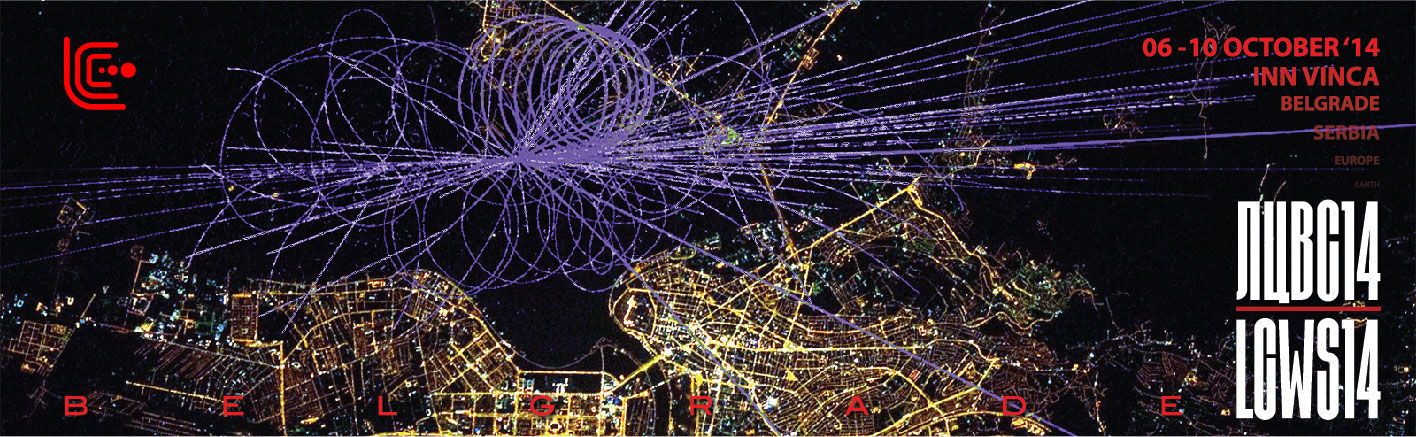
\includegraphics[width=12.8cm,height=6cm,keepaspectratio]{LCWS14.jpg}
  \end{textblock}
  }  
  
% \title{Non-interleaved FFS design}
% \author{Oscar BLANCO$^{1,2}$}
% \institute{LAL$^1$, CERN$^2$}

%% BEGIN Commenting index and first slide
\begin{frame}
\CERNlogo
\LALlogo
% \LCWSlogo
\vspace*{3cm}
\begin{center}
{\LARGE\color{blue} \textbf{Telescope Design}\\BDS Meeting\\Mars 25, 2015}\par
\vspace*{1cm}
Oscar BLANCO$^{1,2}$\par
LAL$^1$, CERN$^2$\par
\end{center}
\end{frame}
% \frame{\titlepage} 
\frame{\frametitle{Table of contents}\tableofcontents}
\section{The Goal}
\begin{frame}{The Goal}
 Minimize the beam size at the IP to recover the luminosity $L$ of a circular accelerator, and limiting the energy loss due to radiation (beamstrahlung) $\delta_{BS}$.
 \begin{equation*}
  L \propto \frac{f_{rep}n_b^2}{\sigma_x\sigma_y}\qquad\delta_{BS}\propto\frac{n_b^2E}{(\sigma_x+\sigma_y)^2}
 \end{equation*}
 {\tiny
 \begin{center}
\begin{tabular}{|l|c||c|c|c|c|}\hline
Parameter & Symbol & LHC & ILC & CLIC 500 GeV& CLIC 3 TeV\\\hline\hline
Energy/z (TeV) & $E$& 7& 0.250 & 0.250 & 1.500\\
Bunch population & $n_b$ &$1.15\times10^{11}$&$2\times10^{10}$&$6.8\times10^9$&$3.72\times10^9$\\
Repetition rate [Hz] &$f_{rep}$& $11.1\times10^{3}$&5 &50&50\\
H/V. IP beam size [nm] & $\sigma_x/\sigma_y$&$16.6\times10^{3}$&474/5.9&202/2.3&40/1\\\hline
E loss (Beamstrahlung) [$\Delta E/E$] &$\delta_{BS}$&-???&0.07&0.07&0.28\\
Luminosity &$L$& $10^{34}$ &$1.57\times10^{34}$ & $2.3\times10^{34}$&$5.9\times10^{34}$\\\hline
\end{tabular}
\end{center}
}
Possible solution : flat beam ($\sigma_x\gg\sigma_y$)
\end{frame}

\section{The problem}
\begin{frame}
 \color{blue}\Large The problem
\end{frame}
\begin{frame}{Chromaticity}
\begin{center}
 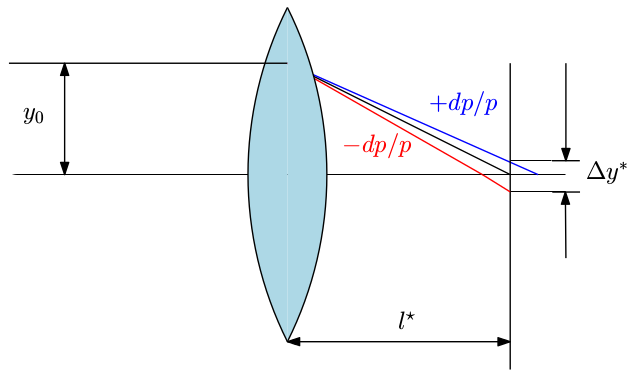
\includegraphics[scale=0.60,angle=0]{chrom.png}
\end{center}
The path length changes as a function of the energy.\par
This generates an increase of the beam size.\par
{\tiny Figure from CERN-THESIS-2014-230.6}
\end{frame}
\section{Why a Telescope ?}
\begin{frame}{Why a telescope ?}
Demagnify the beam with minimal chromaticity generation\par
$x_i=\sum_{j=1}^6R_{ij}x_j+\sum_{j,k=1}^6T_{ijk}x_jx_k+\cdots\qquad x_i\in x,x',y,y',\tau,\delta$\par
\setlength{\TPHorizModule}{1pt}
  \setlength{\TPVertModule}{1pt}
 \begin{textblock}{110}(10,60)
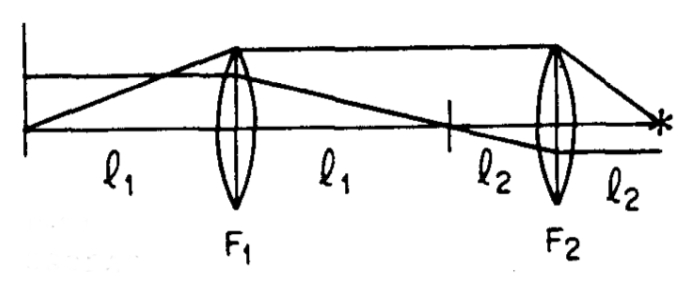
\includegraphics[scale=0.3]{telescope.jpg}
\end{textblock}
\begin{textblock}{110}(180,60)
\begin{equation*}
R=
 \begin{pmatrix}
   M_x & 0 & 0 & 0 \\
   0 & 1/M_x & 0 & 0 \\
   0 & 0 & M_y & 0 \\
   0 & 0 & 0 & 1/M_y \\
  \end{pmatrix}
\end{equation*}
\end{textblock}
\vspace*{2.6cm}
\begin{tcolorbox}[colback=green!5,colframe=green!40!black,title=A Conceptual Design of Final Focus Systems for Linear Colliders]
...$R_{12}(0)=0, T_{116}=0$... 
\begin{equation*}
\beta(\delta)\beta_0 = R_{11}^2\beta_0^2+\boldsymbol{2[0]\delta}+[2R_{11}U_{1166}\beta_0^2+T_{126}^2]\delta^2+\cdots
\end{equation*}
So for telescopic systems ... the derivative with respect to $\delta$ vanishes...\par
... the total chromatic distortion in the triplet system is approximately twice that found in the singlet system !
\end{tcolorbox}
Karl L. Brown (SLAC-PUB-4159)
\end{frame}
\begin{frame}{The problem}
\begin{tcolorbox}[colback=green!5,colframe=green!40!black,title=A Conceptual Design of Final Focus Systems for Linear Colliders]
$\cdots$\par
 The principal problem in designing Final Focusing Systems (FFS) for linear colliders is the elimination or minimization of the chromatic distortions introduced by the final lens system nearest to the interaction point (I.P.).\par
 $\cdots$\par
 There are several possible approaches ...\par
 3. Sextupoles can be introduced into the optical design to cancel the principal second-order chromatic aberrations ...\par
 4. Alternatively one might choose to `live with' the small residual second-order chromatic aberrations\par
 $\cdots$\par
\end{tcolorbox}
Karl L. Brown (SLAC-PUB-4159)
\end{frame}
\subsection{Chromaticity minimization}
\begin{frame}{Chromaticity minimization}
\begin{equation*}
 \xi_x = \frac{1}{\beta_x^*}\left(\cancelto{0}{T_{116}^2}\beta_{x0}+T_{126}^2\frac{1}{\beta_{x0}}\right)\qquad
 \xi_y = \frac{1}{\beta_y^*}\left(\cancelto{0}{T_{336}^2}\beta_{y0}+T_{346}^2\frac{1}{\beta_{y0}}\right)
\end{equation*}
Chromaticity increases the beam size : $\sigma = \sigma^* \sqrt{1+\xi^2\sigma_\delta^2}$
 \setlength{\TPHorizModule}{1pt}
  \setlength{\TPVertModule}{1pt}
\begin{textblock}{400}(120,100)
 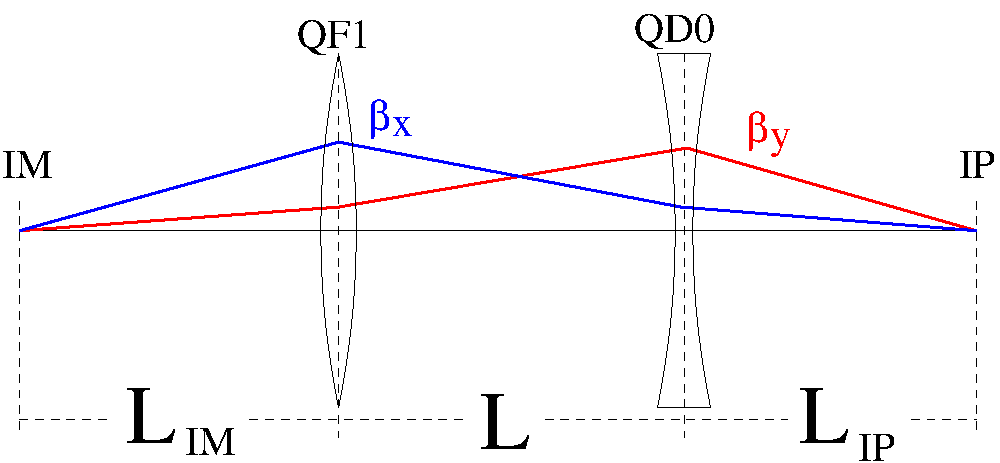
\includegraphics[scale=0.25,angle=0]{fig01.pdf}
\end{textblock} 
\vspace*{2.2cm}
\begin{equation*}
  \xi_{\substack{x\\y}}=\mp\frac{1}{4\pi}\int\beta_{\substack{x\\y}}kdl =\mp\frac{1}{4\pi}\left(\beta_{\substack{x\\y}1}k_1l_1-\beta_{\substack{x\\y}0}k_0l_0\right)
%  \xi_{\substack{x\\y}}
 =\frac{1}{4\pi}\frac{L_{IP}}{\beta^*_{\substack{x\\y}}}\Xi_{\substack{x\\y}}(r,r_{im})
\end{equation*}
with{\tiny
\begin{equation}
 \Xi_{\substack{x\\y}}(r,r_{im})=\mp\sqrt{\frac{1}{rr_{im}}+\frac{1}{r}+\frac{1}{r_{im}}}\sqrt{\frac{1+r/r_{im}}{1+r}}\left[\left(1+r\pm\sqrt{\frac{r}{r_{im}}+r+\frac{r^2}{r_{im}}}\sqrt{\frac{1+r}{1+r/r_{im}}}\right)^2-\left(\frac{1+r}{1+r/r_{im}}\right)\right]
\end{equation}}
$r=L/L_{IP}, r_{im}=L_{IM}/L_{IP}$\par
\end{frame}
\begin{frame}{Chromaticity minimization (cont.)}
\vspace*{8cm}
{\tiny Chromaticity of a doublet in units of $L_{IP}/\beta^*_y$. Example for CLIC 500GeV.}\par
 \setlength{\TPHorizModule}{1pt}
  \setlength{\TPVertModule}{1pt}
  \begin{textblock}{400}(120,80)
 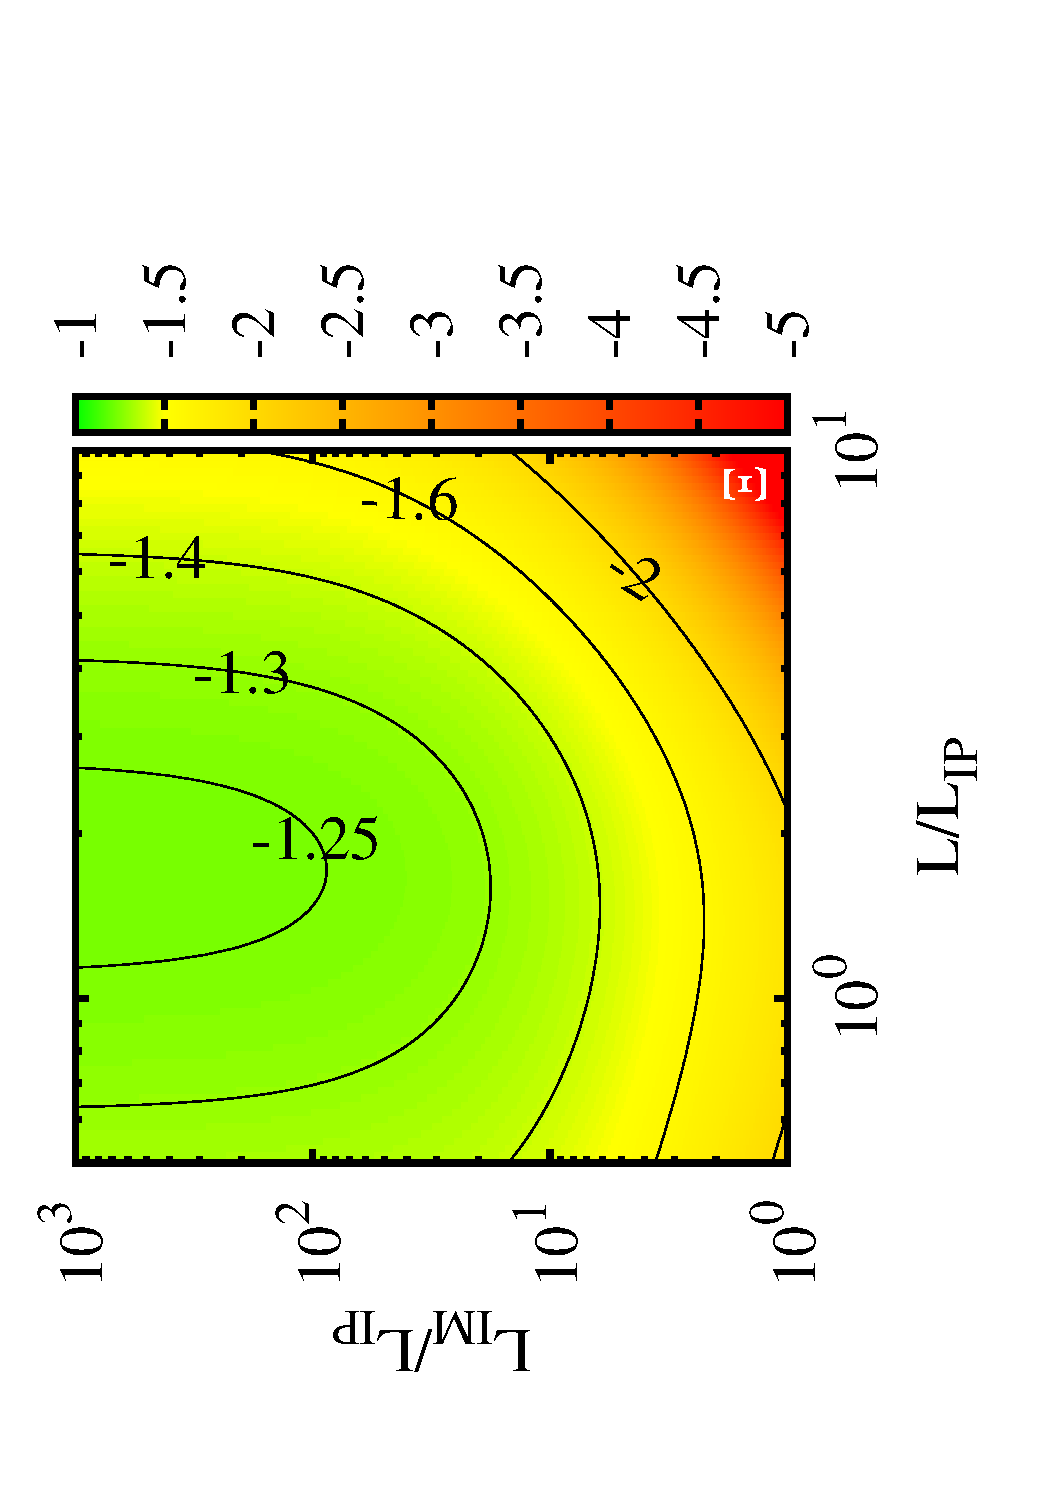
\includegraphics[scale=0.40,angle=-90]{chromHV_500GeVa.pdf}
\end{textblock}
\begin{textblock}{400}(120,25)
 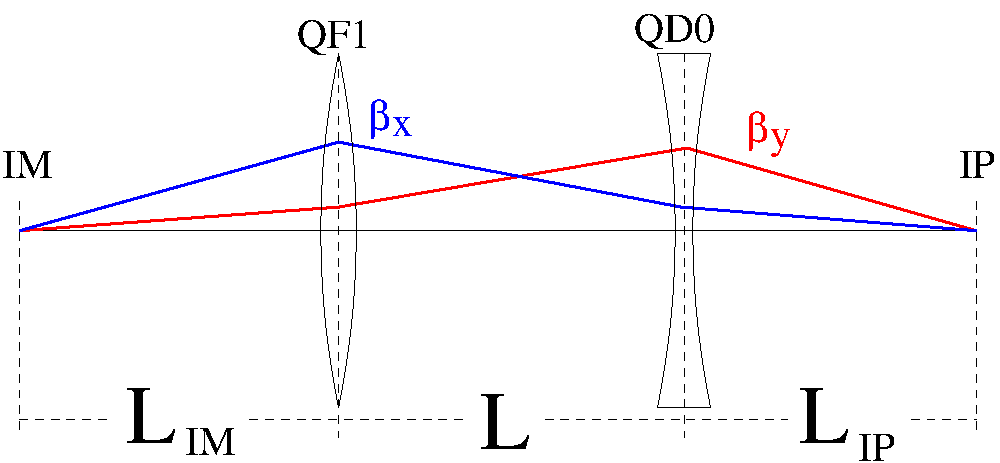
\includegraphics[scale=0.25,angle=0]{fig01.pdf}
 \end{textblock}
 \begin{textblock}{400}(100,60)
 \begin{equation}
  \Xi=\frac{\Xi_x}{\beta_x^*/\beta_y^*}+\Xi_y
 \end{equation}
\end{textblock}
\begin{textblock}{400}(5,75)
 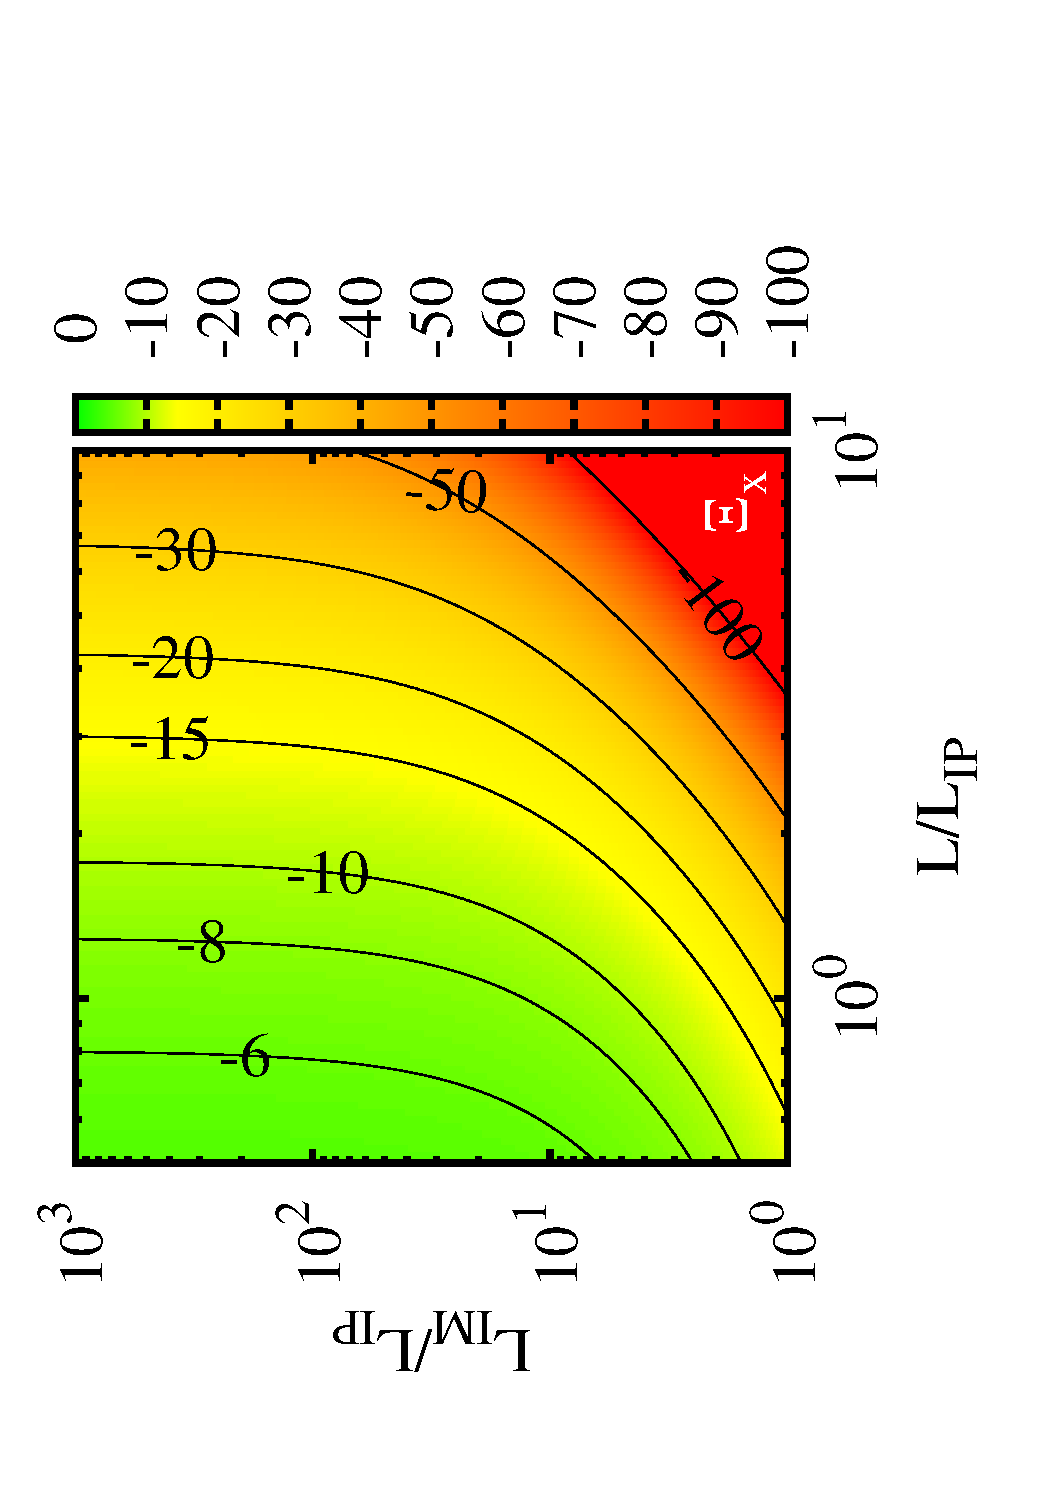
\includegraphics[scale=0.20,angle=-90]{Xi_xa.pdf}
\end{textblock}
\begin{textblock}{400}(5,165)
 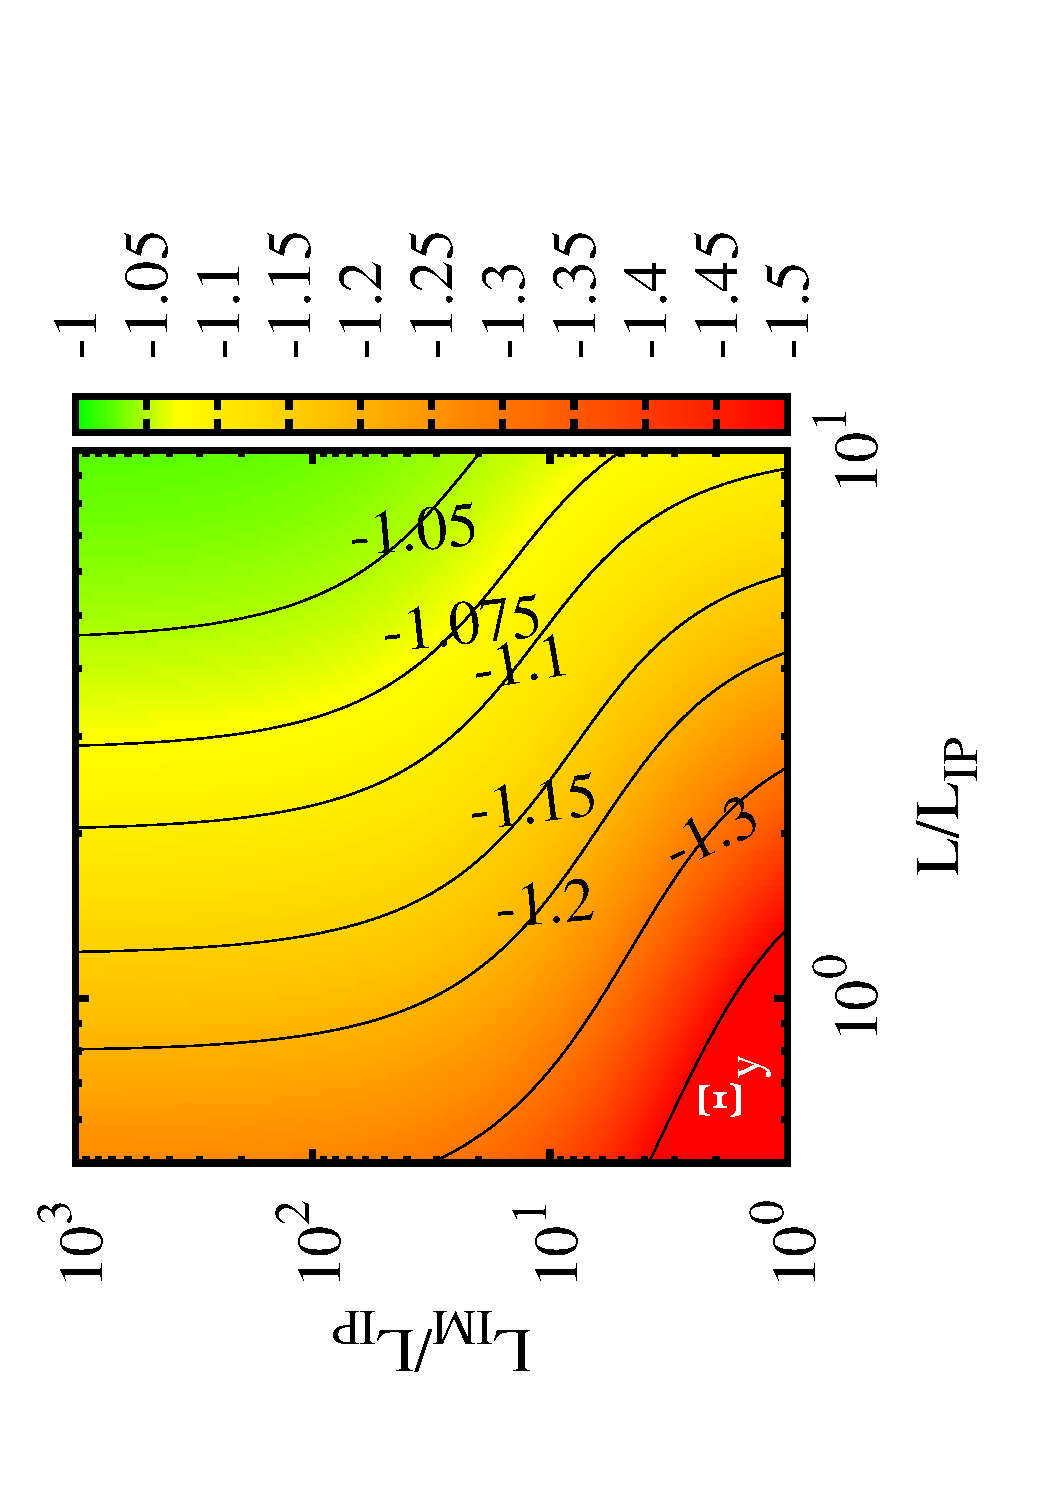
\includegraphics[scale=0.20,angle=-90]{Xi_ya.pdf}
\end{textblock}
\end{frame}
\section{Chromaticity correction}
\subsection{Methods}
\begin{frame}
 \color{blue}\Large Chromaticity correction
\end{frame}
\begin{frame}{Local, Non-local and Non-interleaved correction}
\raggedright
  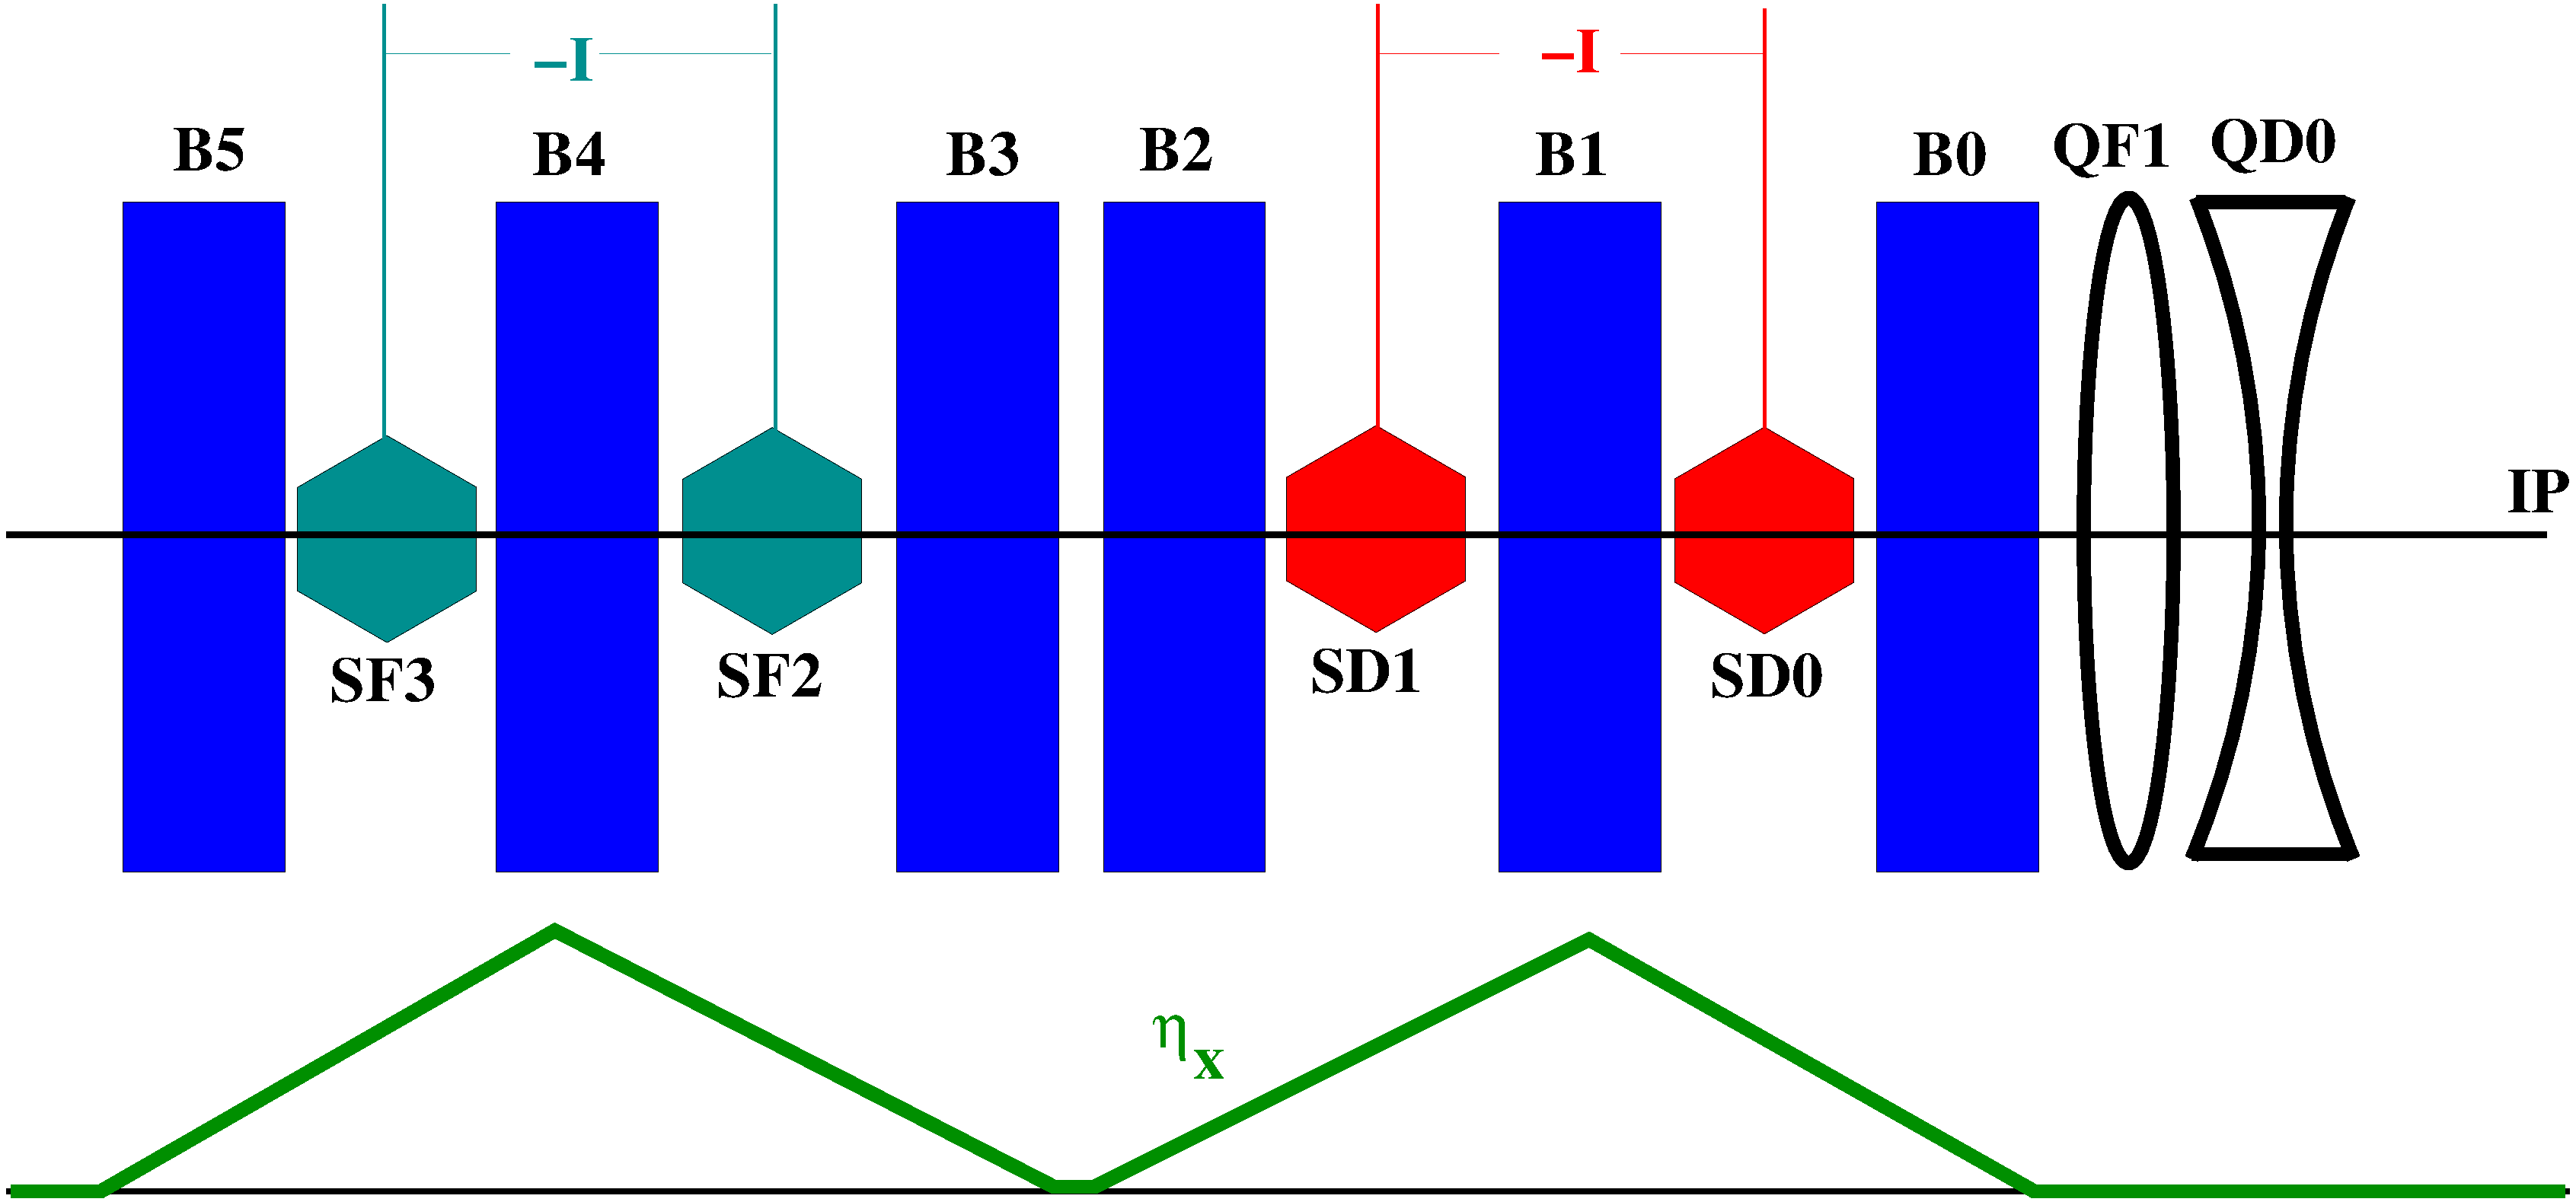
\includegraphics[scale=0.12,angle=0]{nonlocalcorr.pdf}\hspace*{0.5cm}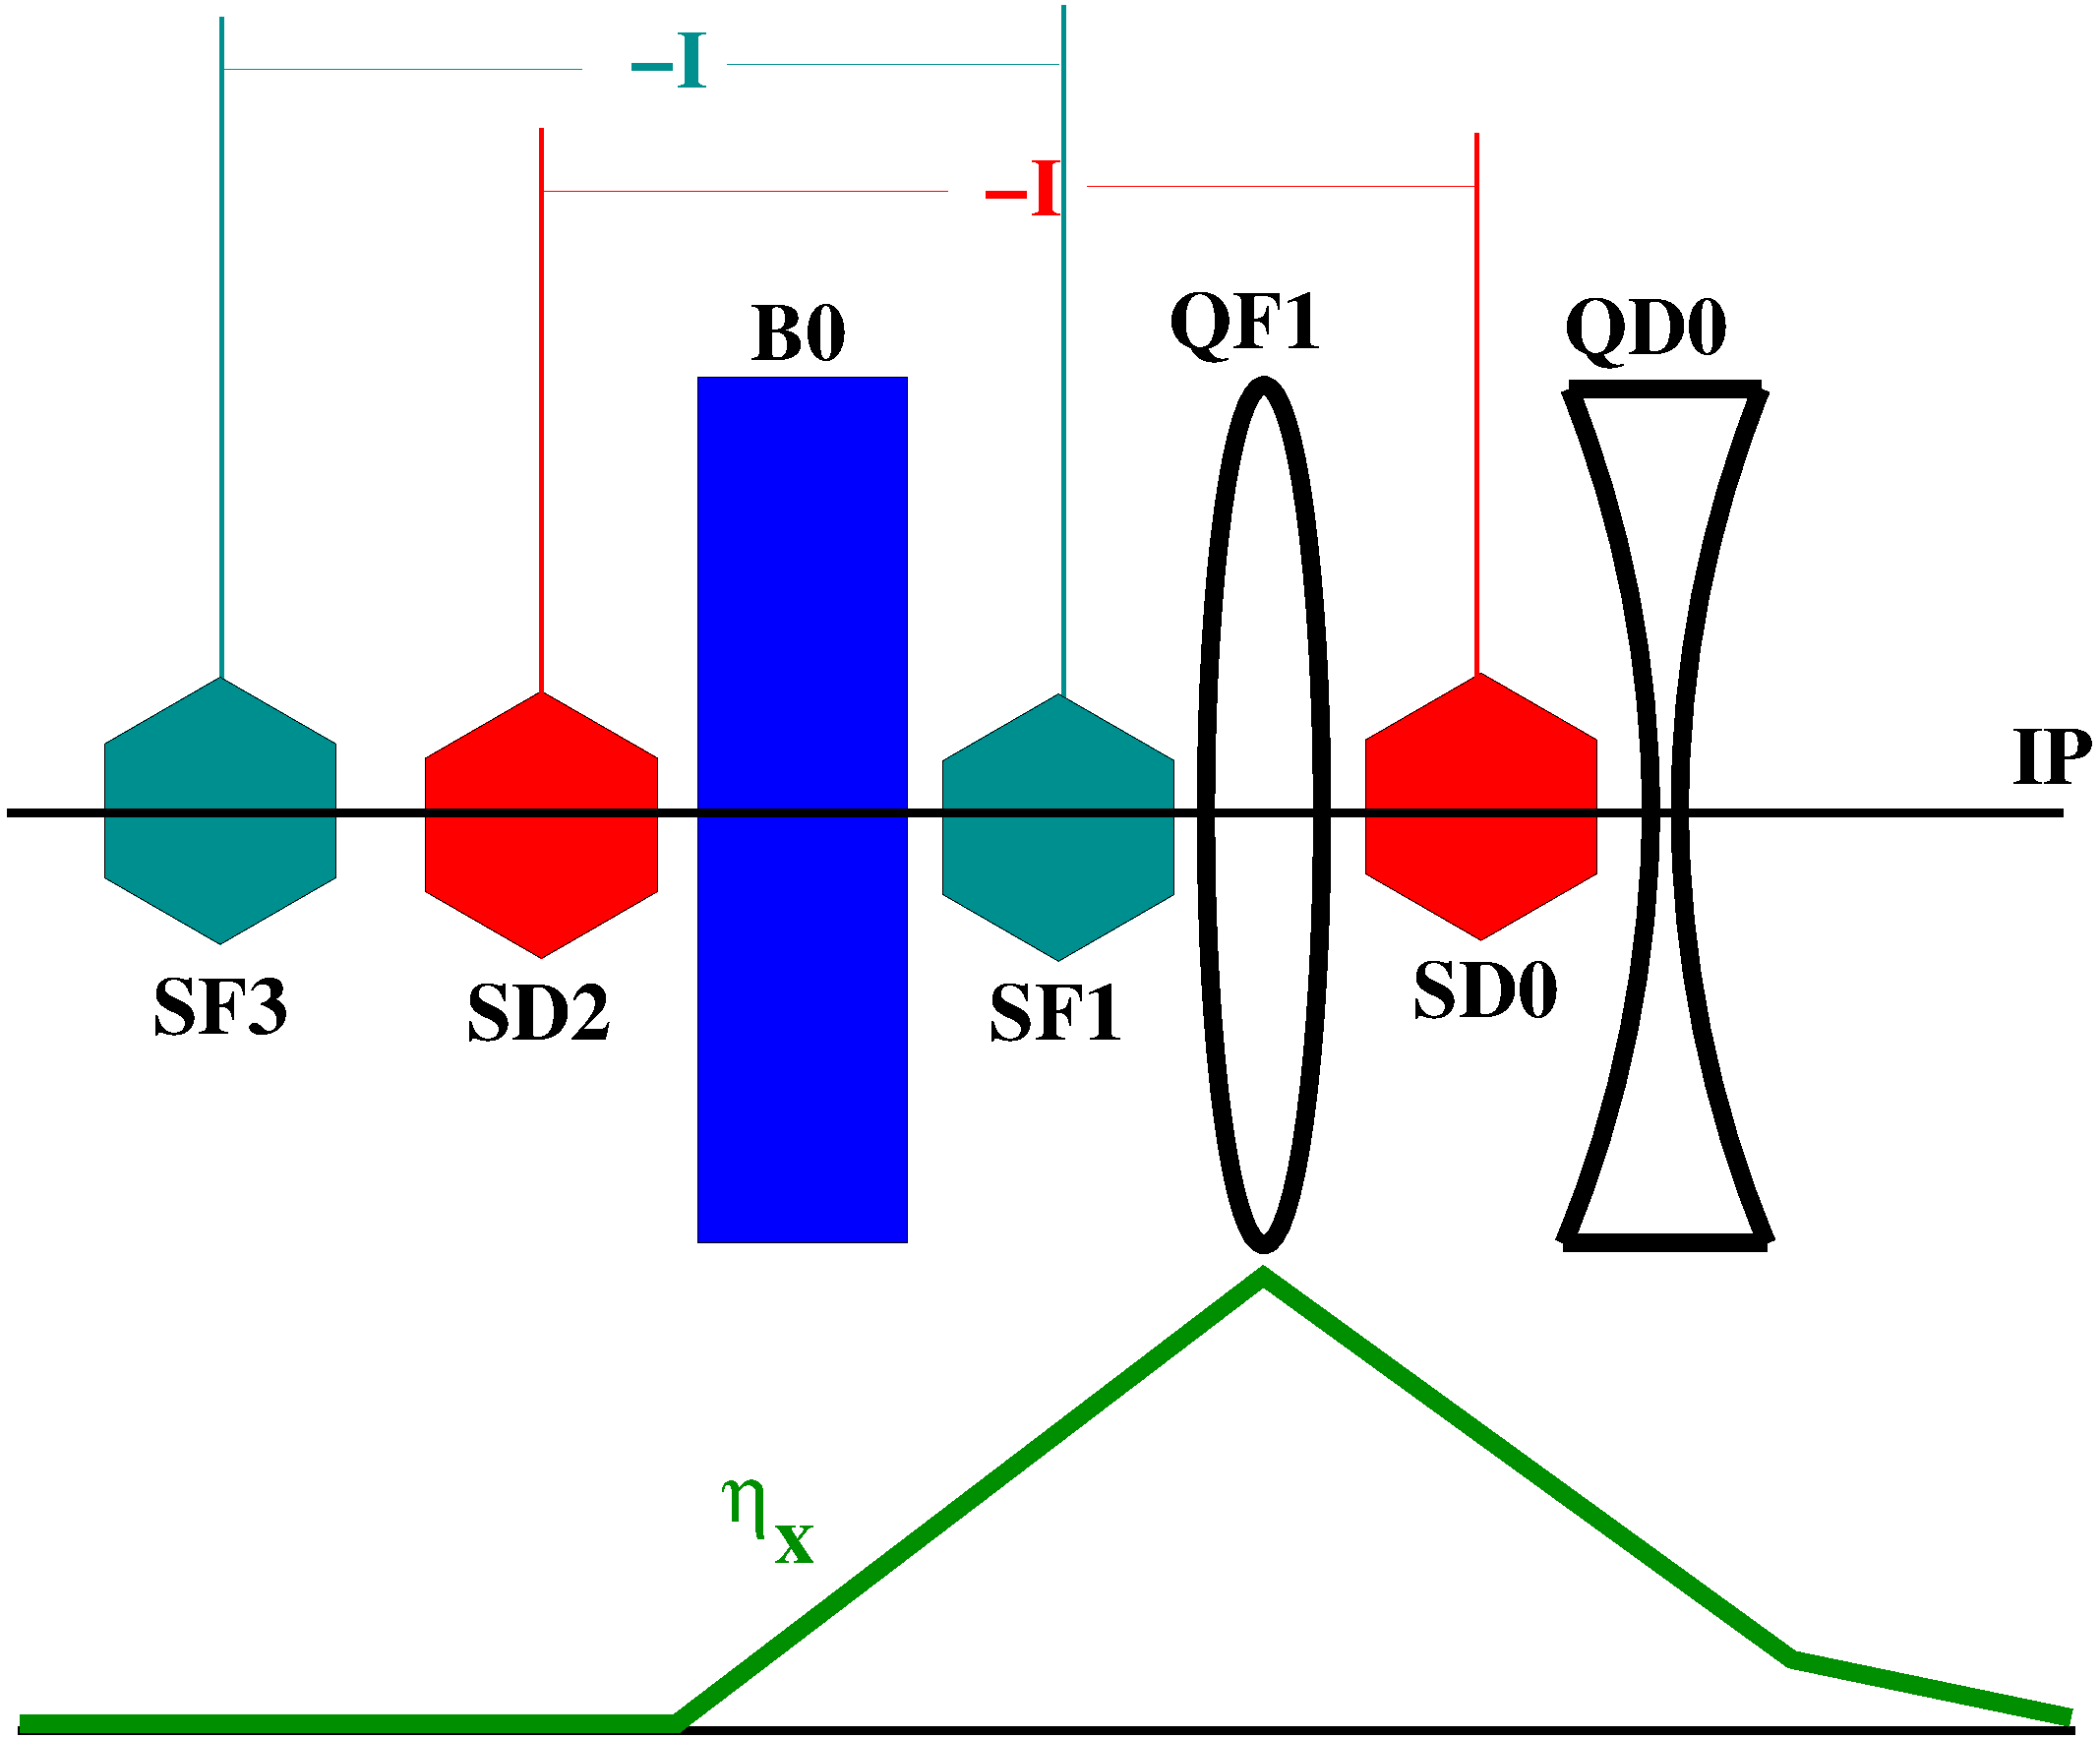
\includegraphics[scale=0.12,angle=0]{localcorr.pdf}\\
  \vspace*{0.5cm}
\centering
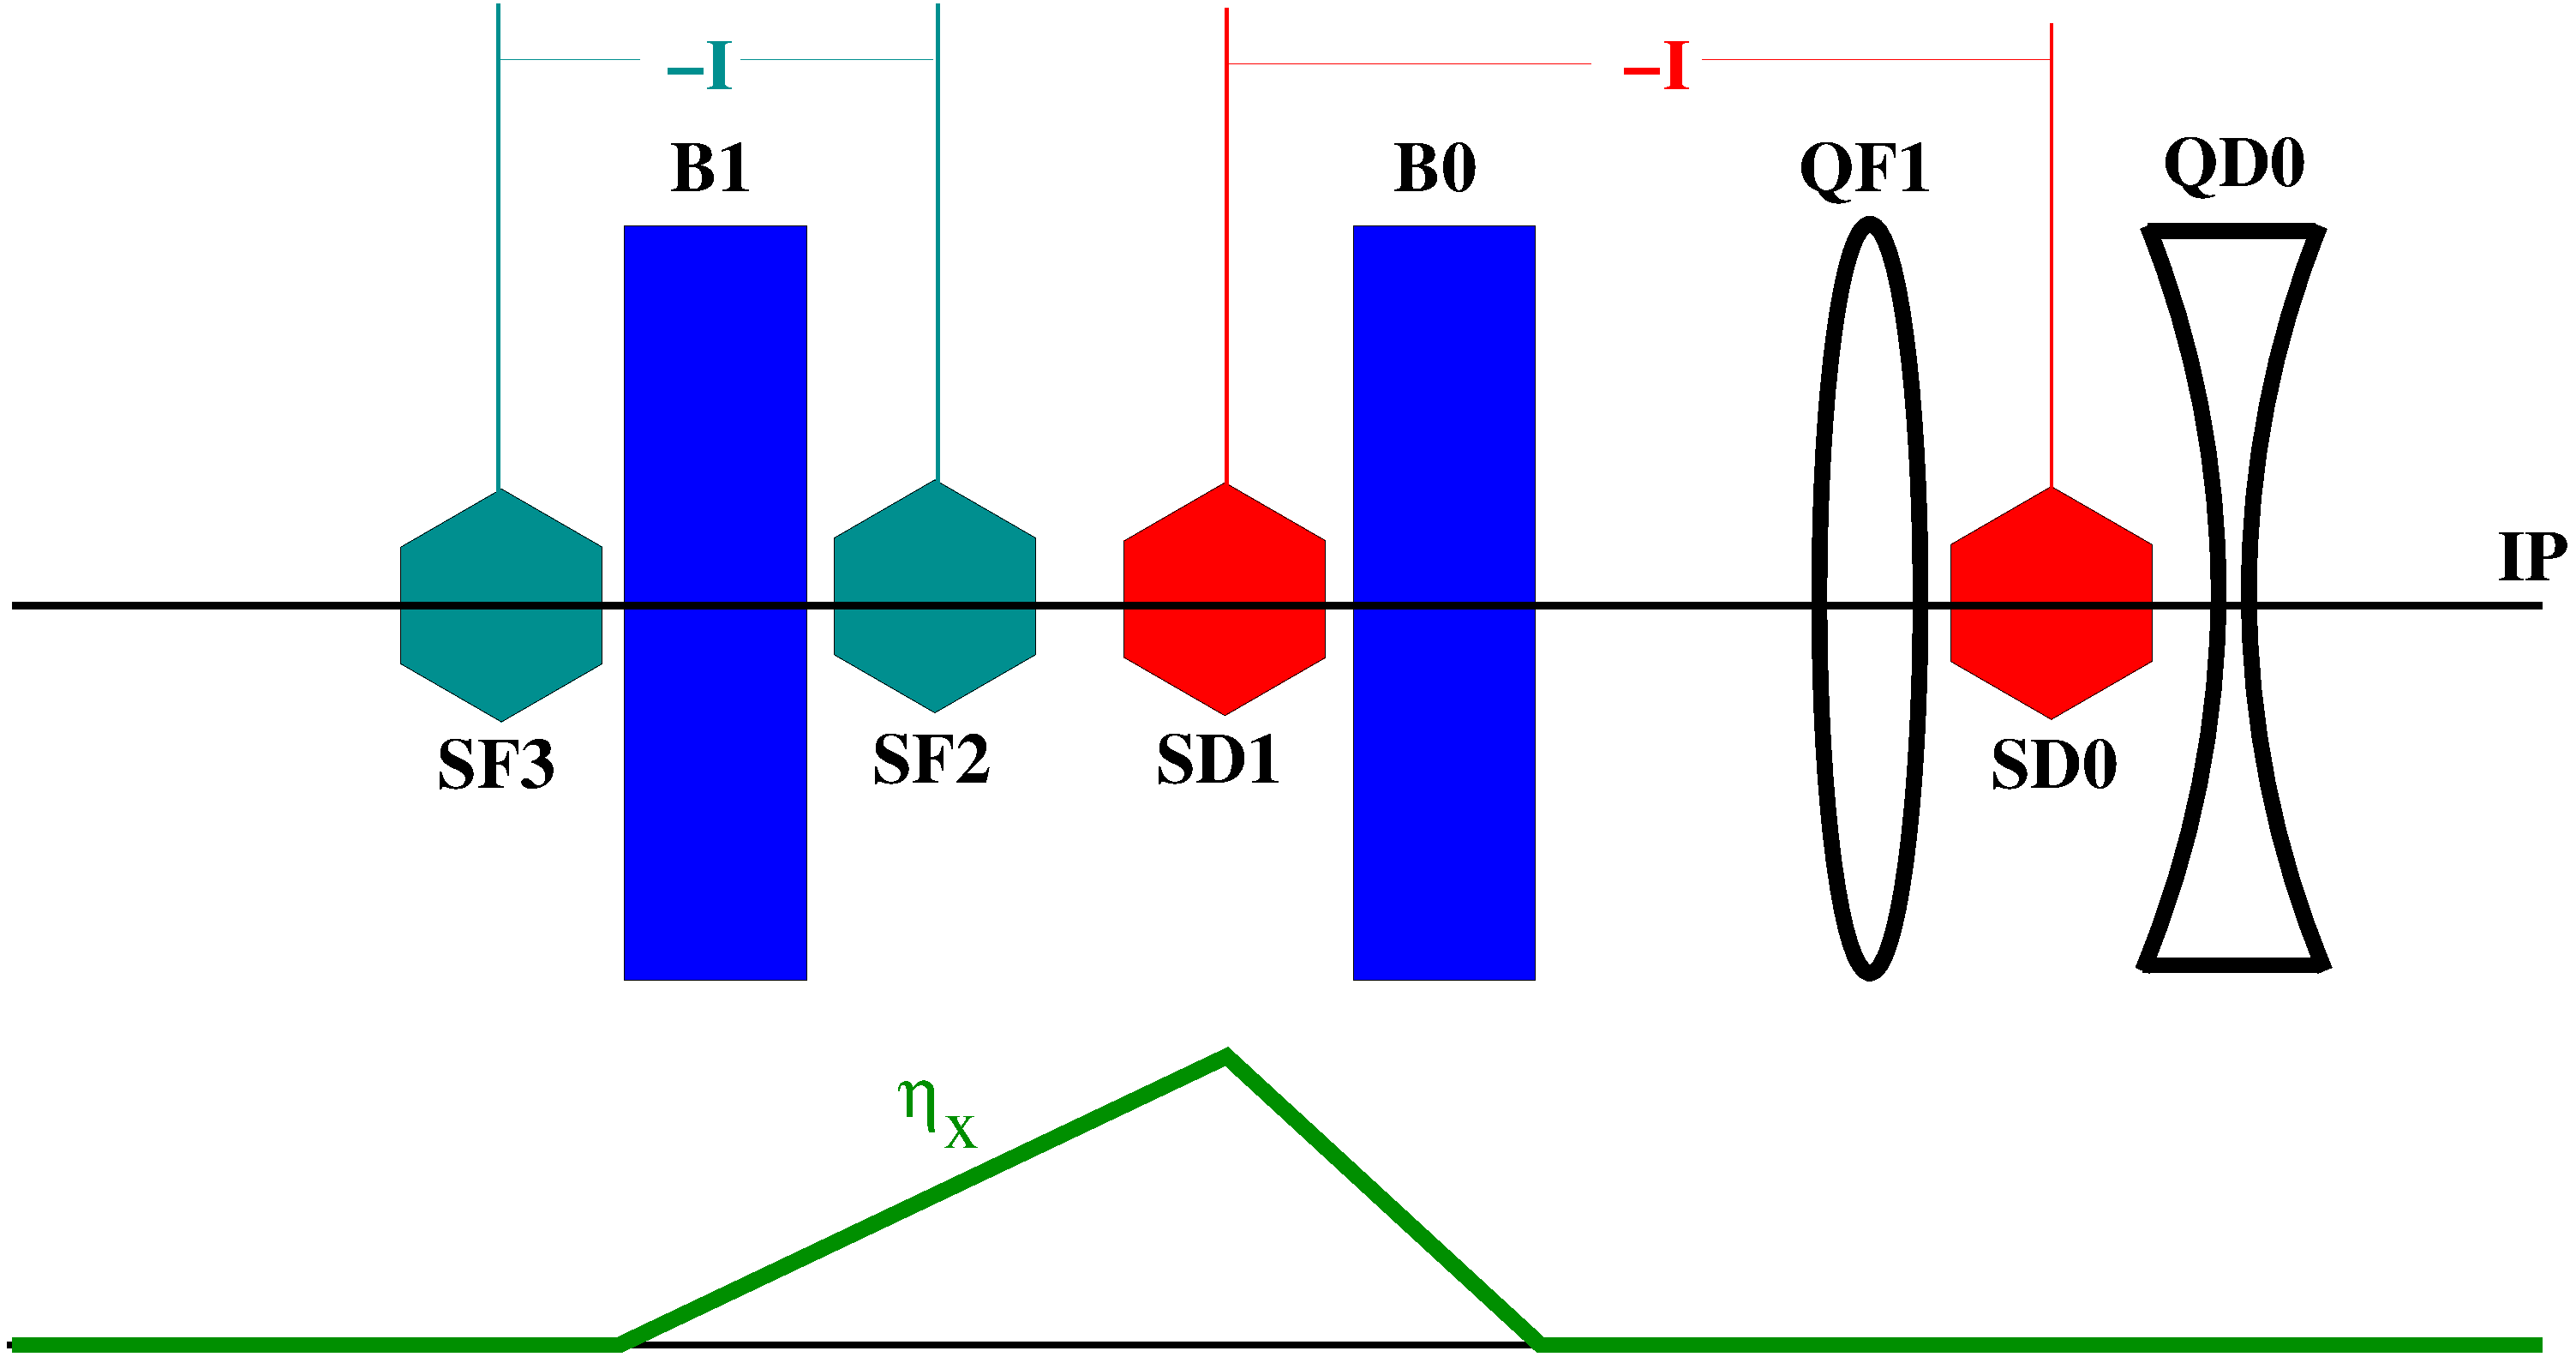
\includegraphics[scale=0.15,angle=0]{noninterleavedcorr.pdf}\\
  \setlength{\TPHorizModule}{1pt}
  \setlength{\TPVertModule}{1pt}
 \begin{textblock}{110}(0,135)
  \textbf{Non-local}
 \end{textblock}
  \begin{textblock}{110}(270,135)
  \textbf{Local}
 \end{textblock}
   \begin{textblock}{110}(220,240)
  \textbf{Non interleaved}
 \end{textblock}
\end{frame}
% \section{Some design criteria}
% \begin{frame}
%  \color{blue}\Large Some design criteria
% \end{frame}
% \subsection{Zero dispersition and beam waist}
% \begin{frame}{Zero dispersition}
% Here, $x$ is any of the two transverse coordinates\par
%  $x = x_\beta+\eta\delta$\par
%  Ideally $\eta=0$ at the IP\par
%  \begin{equation}
%   \sigma = \sigma_\beta^2\left(1+\frac{\eta^2\sigma_\delta^2}{\sigma_\beta}\right)
%  \end{equation}
%  \begin{equation}
%   \frac{\eta\sigma_\delta}{\sigma_\beta}<1\text{@IP}
%  \end{equation}
%  $\sigma_\delta$ is the second moment of the $\delta$ distribution\par
%  \vspace*{0.4cm}
%  {\color{blue}\Large Beam waist}\par
% The beam waist ($\alpha=0$) is at the IP\par
% \begin{equation}
%  \beta(s)=\beta^*+\frac{s^2}{\beta^*}\qquad \alpha=-\frac{s}{\beta^*}
% \end{equation}
% Normally $\alpha<1$, ($10^{-2\sim-3}$), is OK.
% \end{frame}
% \subsection{Oide effect}
% \begin{frame}{Oide effect (Solved in MAPCLASS2)}
%  For the vertical plane,
%  \begin{equation}
%   \sigma^2_{oide} = \frac{110}{3\sqrt{6\pi}}r_e\frac{\lambda_e}{2\pi}\gamma^5 F(\sqrt{k}L,\sqrt{k}l^*)\left(\frac{\epsilon}{\beta^*}\right)^{5/2}
%   \label{Oideequ}
%  \end{equation}
%  where
%  {\small
%  \begin{equation}
%   F(\sqrt{k}L, \sqrt{k}l^*) = \int_0^{\sqrt{k}L}|\sin\phi+\sqrt{k}l^*\cos\phi|^3\left[\int_0^\phi(\sin\phi'+\sqrt{k}l^*\cos\phi')^2 d\phi'\right]^2d\phi
%   \label{OideF}
%  \end{equation}}
%  Oide effect at the Final Doublet is negligible for 500 GeV\par
%  \vspace*{5cm}
%  \setlength{\TPHorizModule}{1pt}
%   \setlength{\TPVertModule}{1pt}
%  \begin{textblock}{400}(25,160)
%  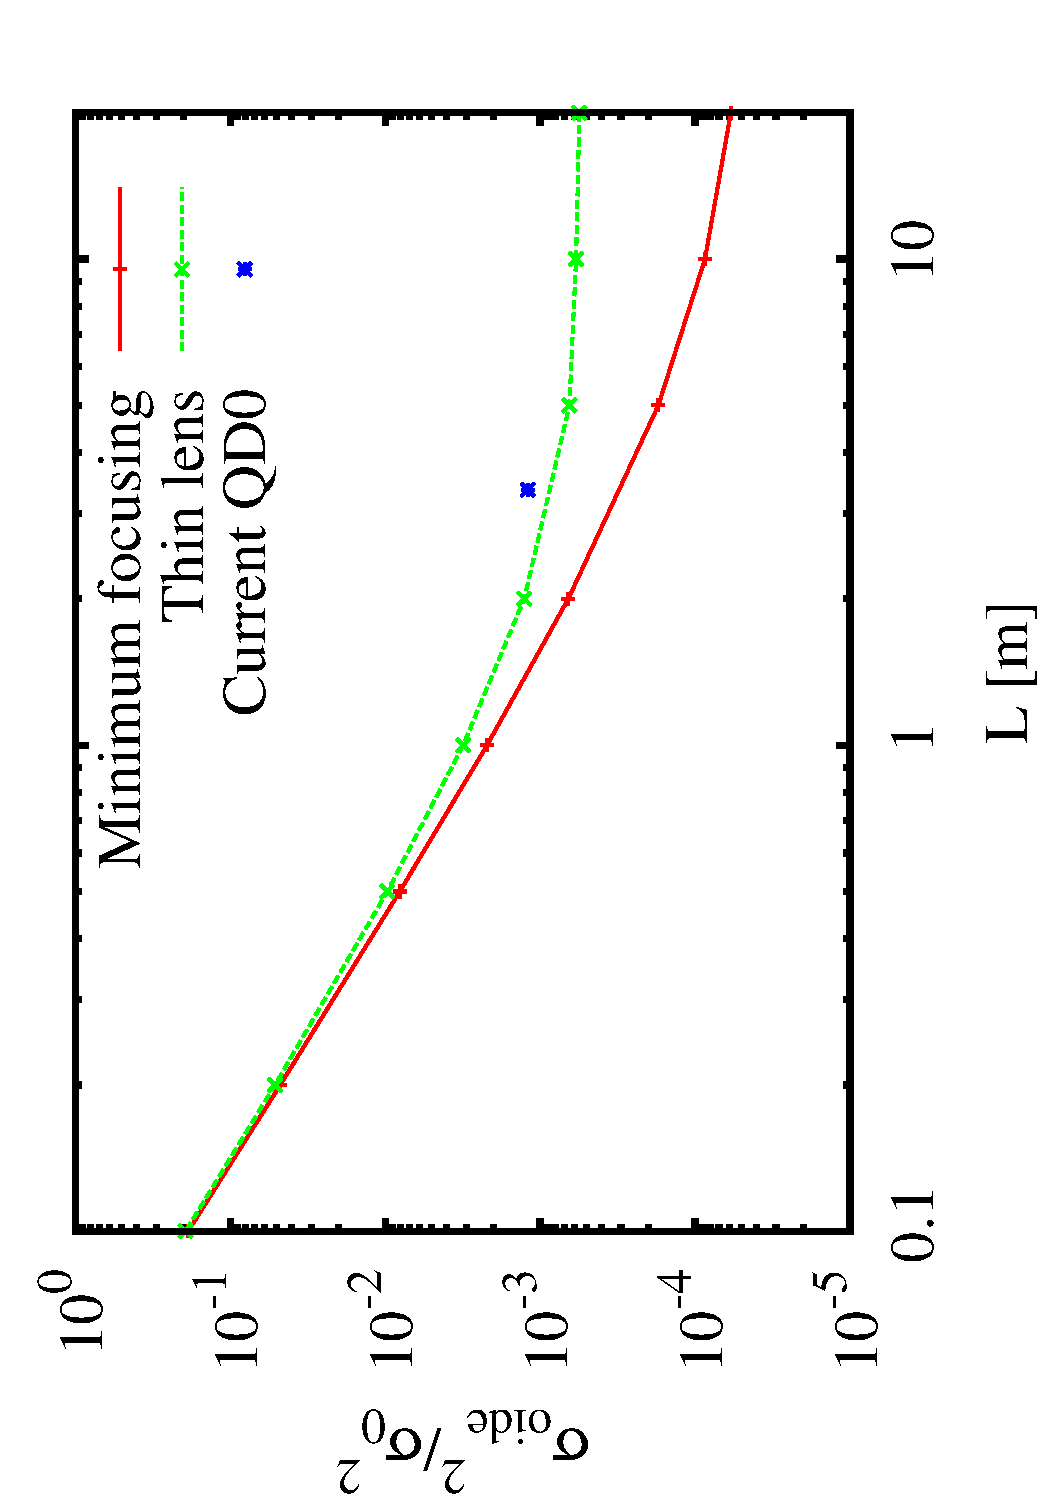
\includegraphics[scale=0.22,angle=-90]{image06b.pdf}
%  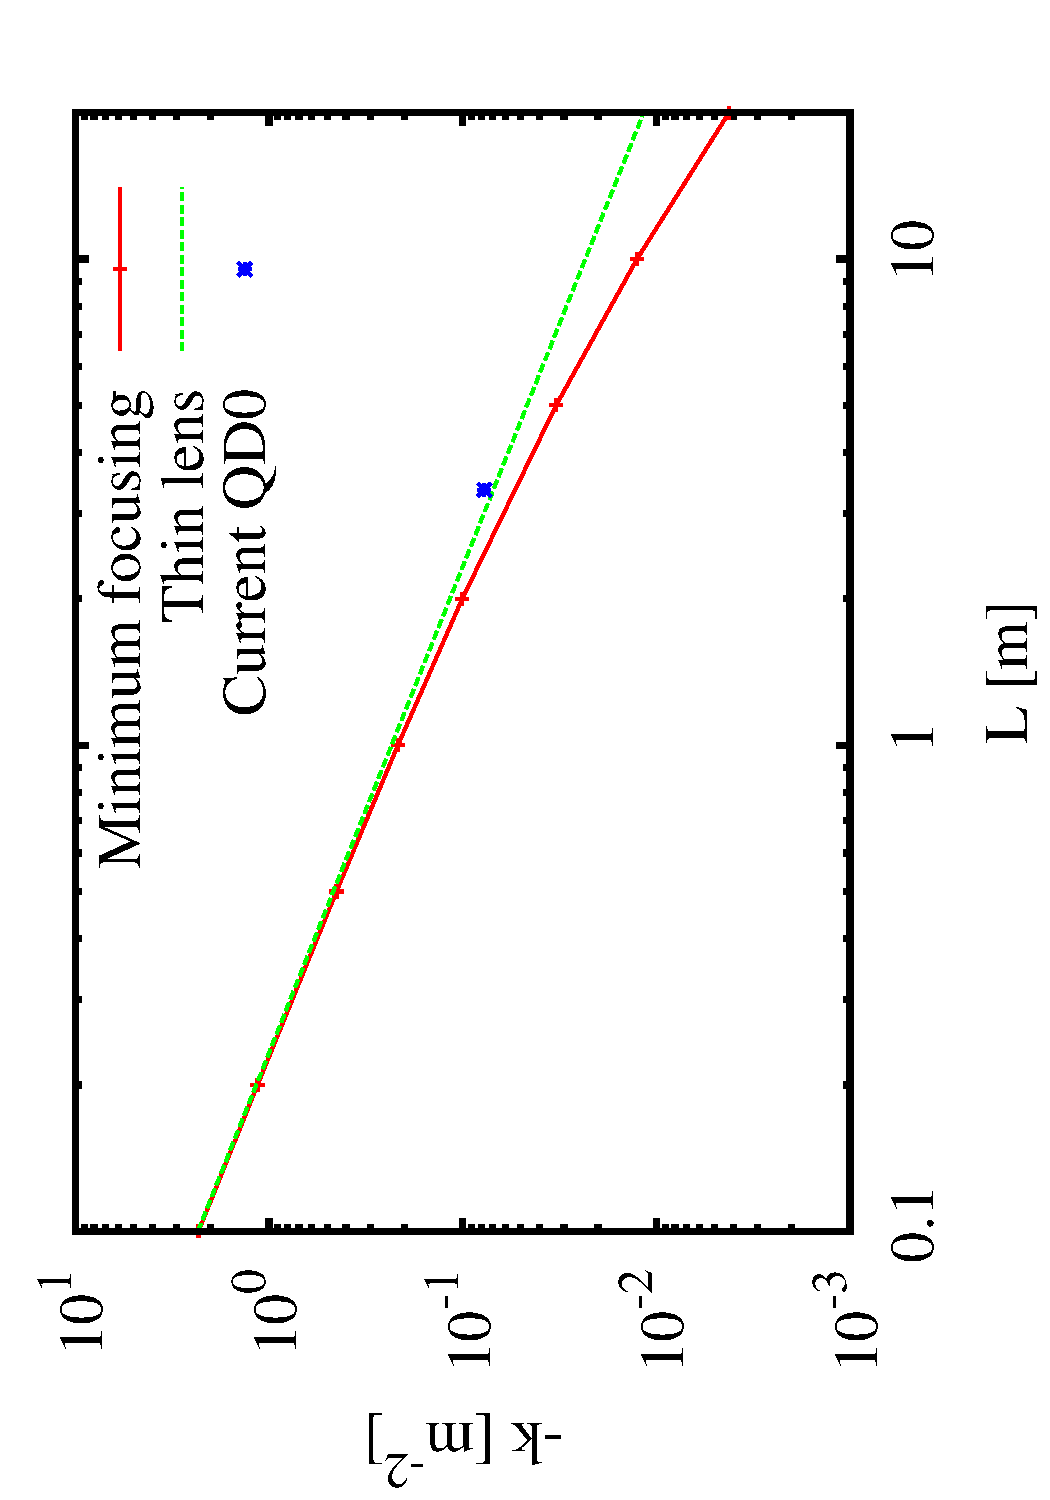
\includegraphics[scale=0.22,angle=-90]{image06c.pdf}
% \end{textblock}
% \end{frame}
\subsection{Second order terms reduction}
\begin{frame}{Second order terms reduction}\,
  {\scriptsize Quadrupoles generate chromaticity ($k_1 \delta x, k_1 \delta y$) and in dispersive regions also generate second order dispersion ($k_1\eta_x\delta^2$).\par
  One of the paired sextupoles is in a horizontal dispersive region ($\eta_x\neq0$).\par
  This will correct second order dispersion ($\eta_x^2\delta^2$), twice the h. chromaticity ($\eta_x\delta x_1$) and the total v. chromaticity ($\eta_x\delta y$).\par
  The sextupoles in non-dispersive regions ($\eta_x=0$) will correct the geometrical components from sextupoles ($x^2, y^2, xy$).\par
  }
  \begin{align*}
   x'_2 = & \frac{k_2}{2}(x_1+\eta_x\delta)^2-y_1^2=\frac{k_2}{2}(x_1^2+2x_1\eta_x\delta+\eta_x^2\delta^2-y_1^2)\\
   y'_2 = & k_2 (x_1+\eta_x\delta)y = k_2 (x_1y_1 +\eta_x\delta y_1)
  \end{align*}

% To minimize their impact on the beam size, the phase advance from the sextupole in the dispersive region to the IP must be $(2n+1)\pi/2$.
%  \setlength{\TPHorizModule}{1pt}
%   \setlength{\TPVertModule}{1pt}
%   \begin{textblock}{400}(120,30)
 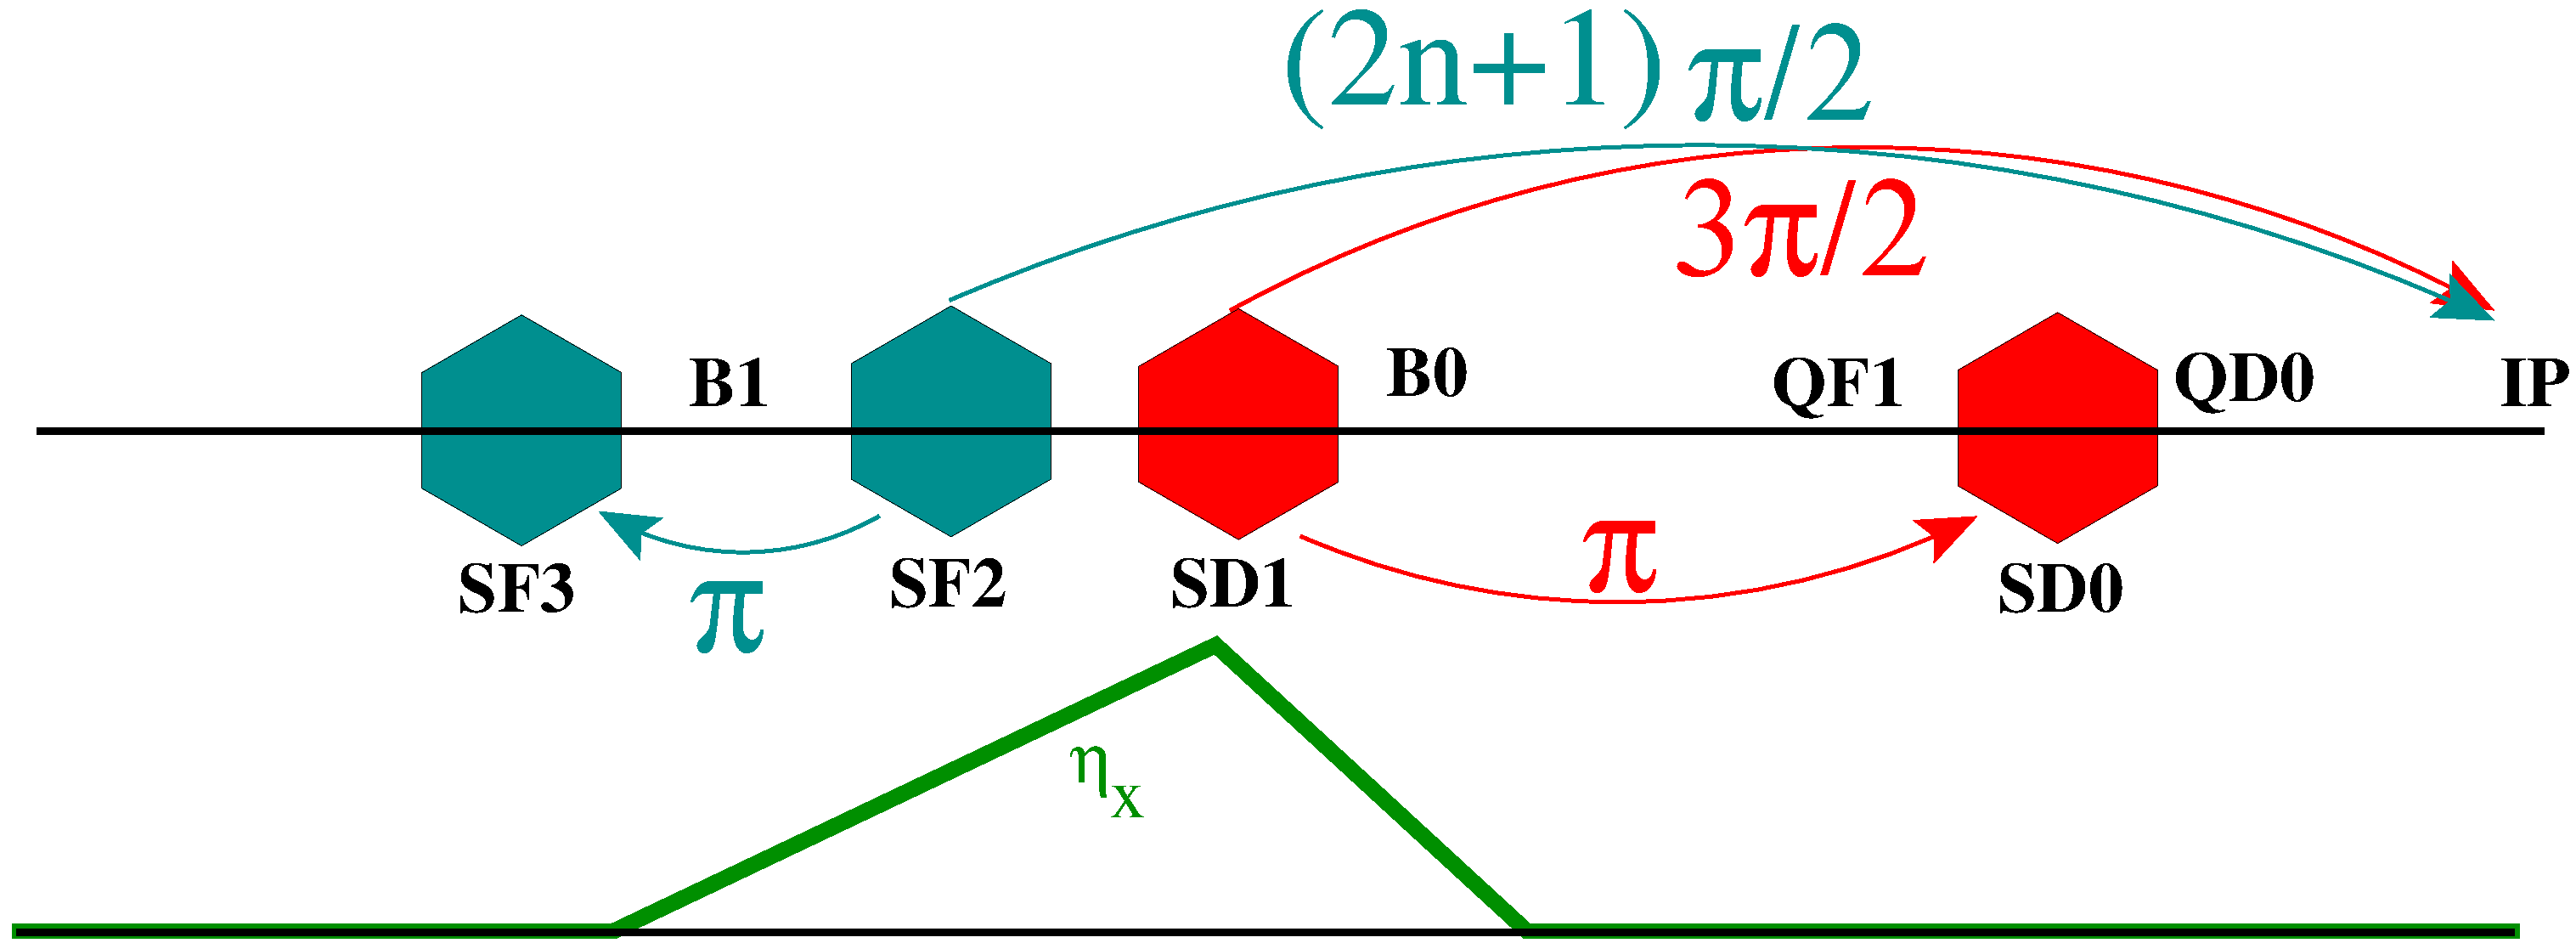
\includegraphics[scale=0.20,angle=0]{phase_adv.pdf}\par
% \end{textblock}
% {\Large  \color{blue}Radiation in bending magnets}
%  \begin{equation*}
% \sigma^2_{bend} \propto\int_0^{IP} \frac{E^5}{\rho^3}t_{16}(s,IP)^2 ds\label{eq-R16}
% \end{equation*}
% {\small Enough dispersion to cancel chromaticity but not to much due to radiation.}
\end{frame}
\begin{frame}{geometrical terms}
 \setlength{\TPHorizModule}{1pt}
  \setlength{\TPVertModule}{1pt}
  \begin{textblock}{400}(120,30)
 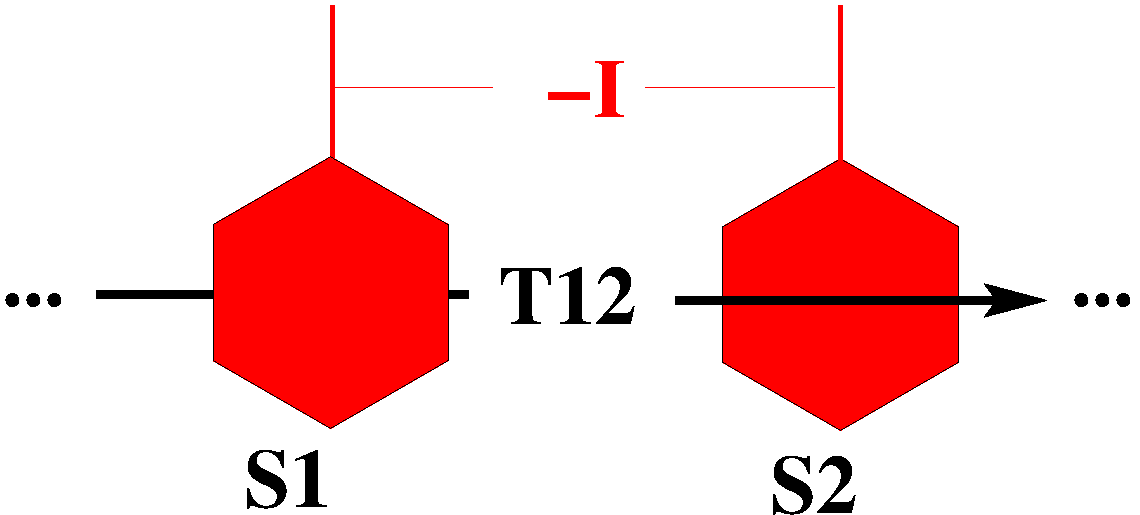
\includegraphics[scale=0.20,angle=0]{geo_cancel.pdf}
\end{textblock}
  \begin{textblock}{200}(140,90)
 Ideally the phase\par
 advance is $\pi$.
%  $\Delta\phi$ represents the phase advance {\color{red}error}.
 \end{textblock}
 \begin{textblock}{200}(10,150)
%  Ideally the phase advance is $\pi$.
 $\Delta\phi$ represents the phase advance {\color{red}error}.
 \end{textblock}
  \begin{textblock}{100}(5,70)
  \begin{equation*}
 T_{12}=
  \begin{pmatrix}
   t_{11} & t_{12} & 0 & 0 \\
   t_{21} & t_{22} & 0 & 0 \\
   0 & 0 & t_{33} & t_{34} \\
   0 & 0 & t_{43} & t_{44} \\
  \end{pmatrix}
 \end{equation*}
 \end{textblock}
   \begin{textblock}{100}(220,70)
  \begin{equation*}
 \rightarrow
  \begin{pmatrix}
   M_x & 0 & 0 & 0 \\
   t_{21} & 1/M_x & 0 & 0 \\
   0 & 0 & M_y & 0 \\
   0 & 0 & t_{43} & 1/M_y \\
  \end{pmatrix}
 \end{equation*}
 \end{textblock}
 \begin{textblock}{200}(10,150)
 \begin{align*}
t_{11}t_{22}=&1-{\color{red}(\alpha_{x2}-\alpha_{x1})\Delta\phi_x}\\
t_{33}t_{44}=&1-{\color{red}(\alpha_{y2}-\alpha_{y1})\Delta\phi_y}\\
t_{12} =& {\color{red}\sqrt{\beta_{x1}\beta_{x2}}\Delta\phi_x}\\
t_{34} =& {\color{red}\sqrt{\beta_{y1}\beta_{y2}}\Delta\phi_y}\\
  &\text{and}\\
  0 =& {\color{red}\beta_{y2}/\beta_{y1}-\beta_{x2}/\beta_{x1}}
\end{align*}
\end{textblock}
 \begin{textblock}{150}(210,150)
  \vspace*{0.5cm}
  $\alpha\Delta\phi\ll 1$\par
  $M>1, \beta\Delta\phi<1$\par
  $M_x-M_y\ll1$, it will set a limit to the cancellation of geometrical terms in both planes at the same time, when matching the sextupoles.\par
 \end{textblock}
\end{frame}
% \begin{frame}{$-I$ transformation (geometrical terms cancelled (cont.))}
%  If $\left(\frac{\beta^*}{L_{IP}}\right)^2\ll1$, then, the beta functions are
% \begin{align}
%  \beta_{\substack{x\\y}0}=\frac{L^2_{IP}}{\beta^*_{\substack{x\\y}}},\qquad \beta_{\substack{x\\y}1}&=\beta_{\substack{x\\y}0}\left(1+r\pm\sqrt{\frac{r}{r_{im}}+r+\frac{r^2}{r_{im}}}\sqrt{\frac{1+r}{1+r/r_{im}}}\right)^2
% \end{align}
% \setlength{\TPHorizModule}{1pt}
%   \setlength{\TPVertModule}{1pt}
% \begin{textblock}{400}(120,25)
%  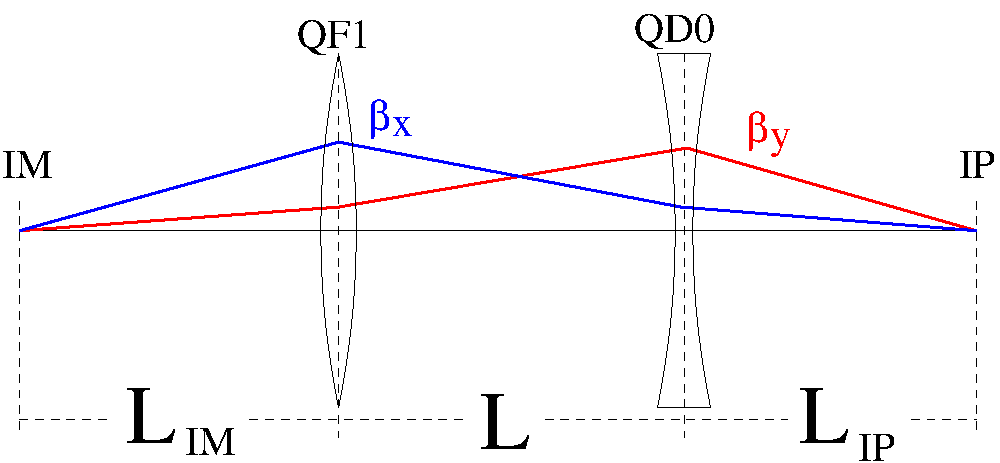
\includegraphics[scale=0.25,angle=0]{fig01.pdf}
% \end{textblock}
% \begin{textblock}{400}(170,165)
%  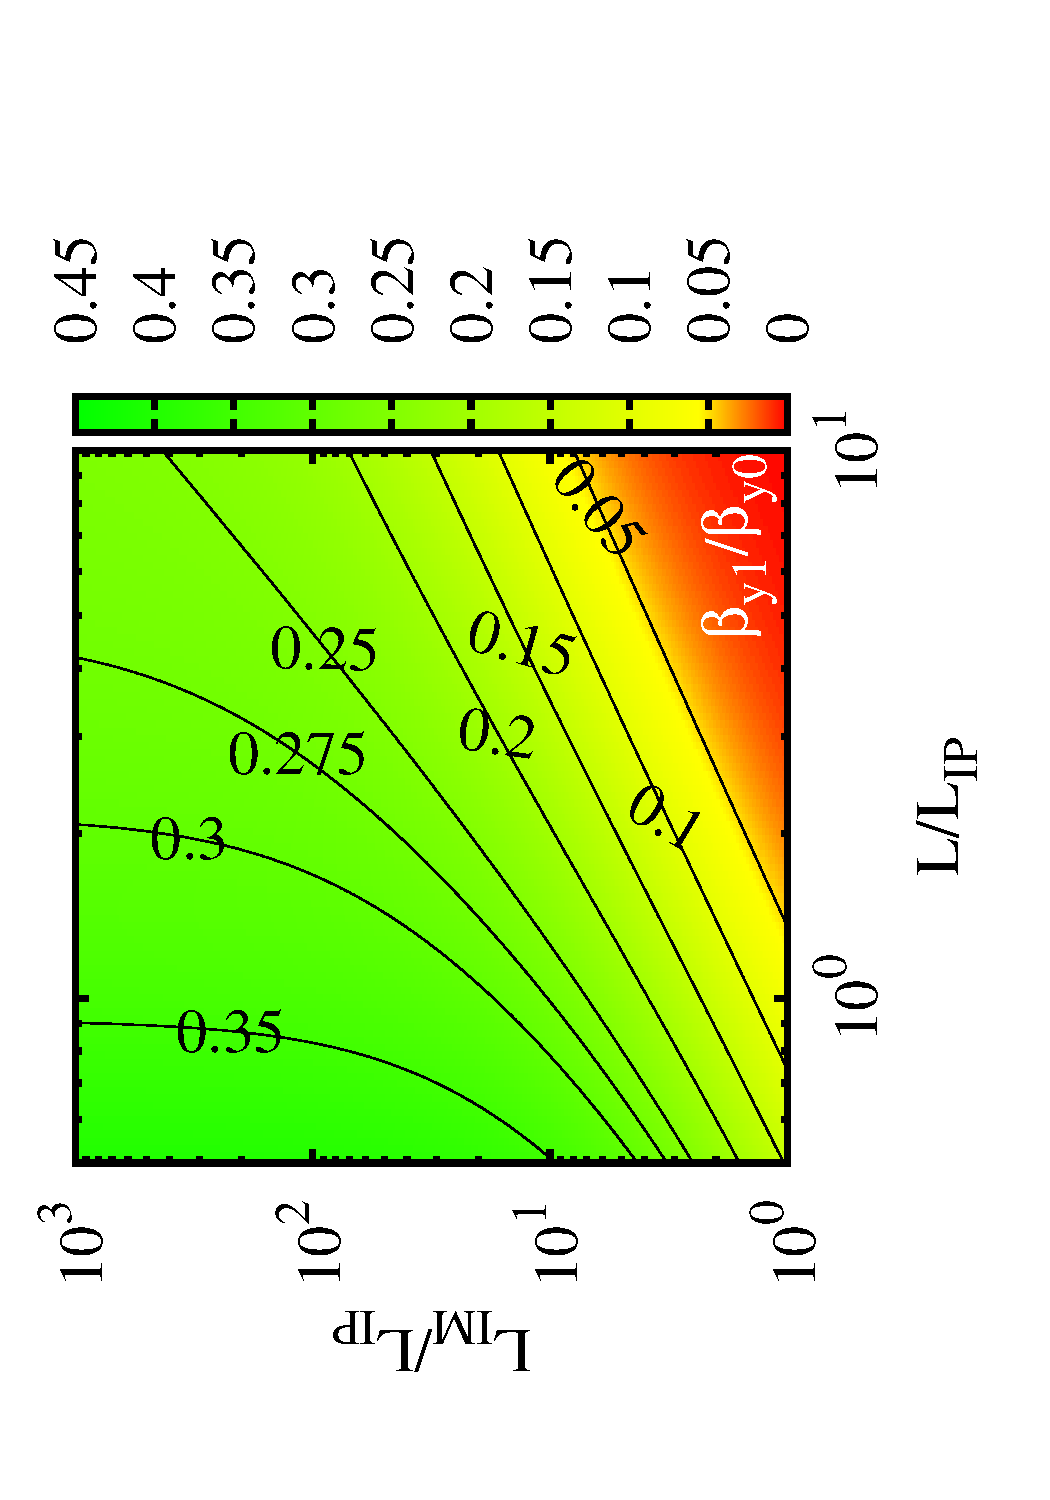
\includegraphics[scale=0.20,angle=-90]{betay1a.pdf}
% \end{textblock}
% \begin{textblock}{400}(5,165)
%  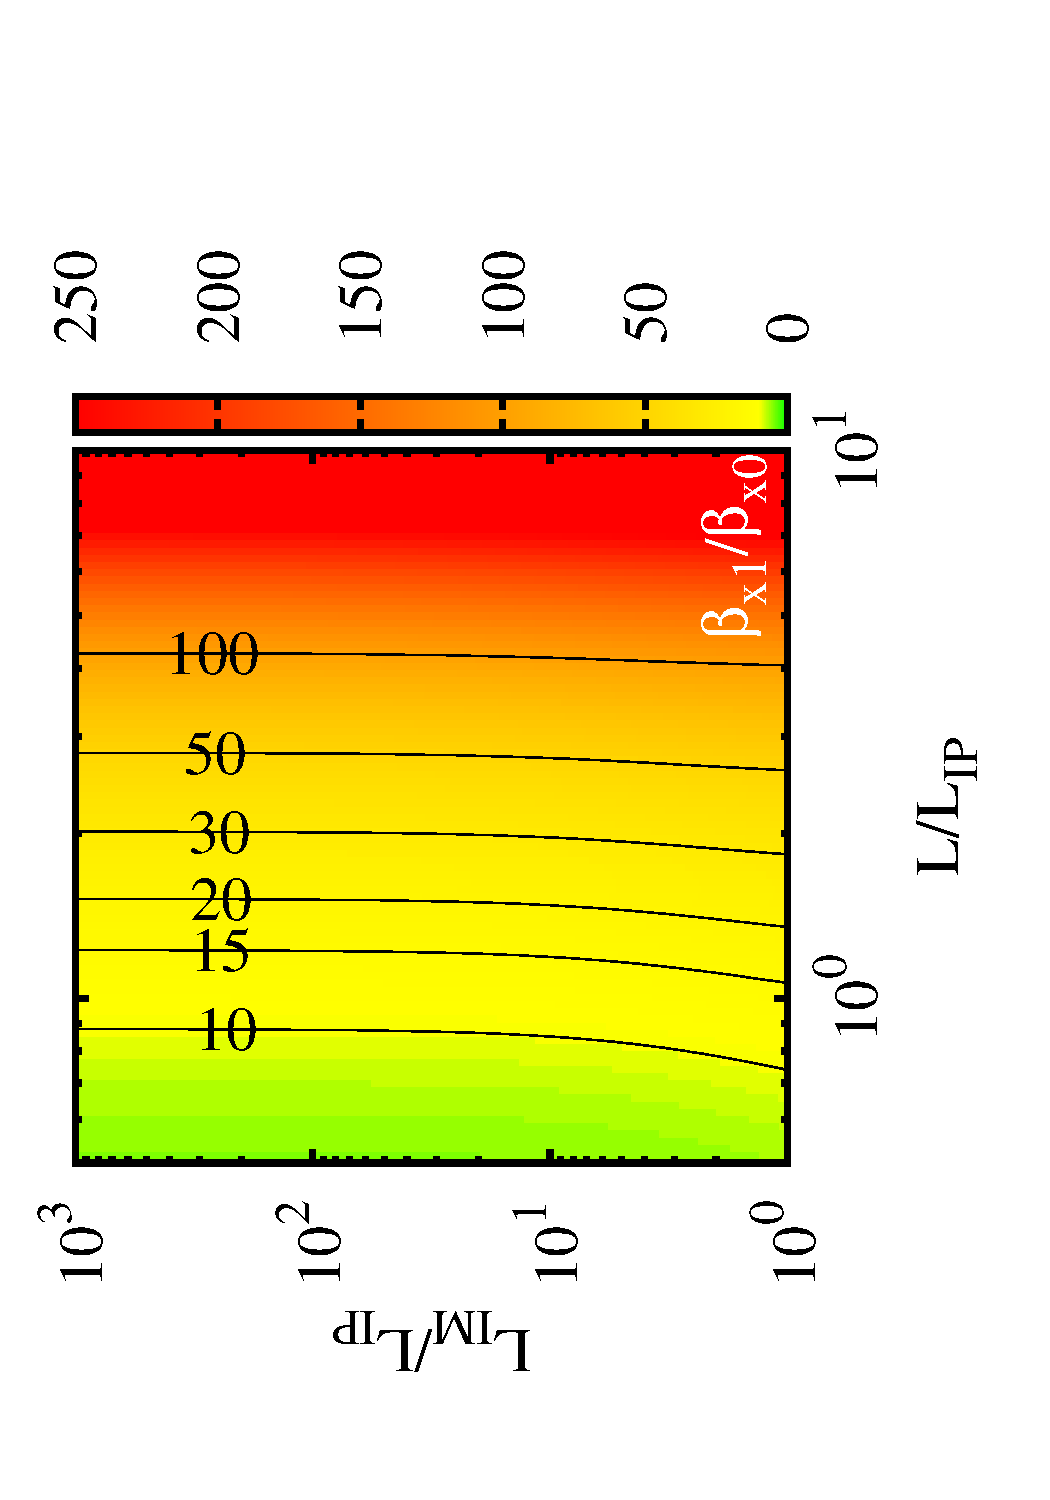
\includegraphics[scale=0.20,angle=-90]{betax1a.pdf}
% \end{textblock}
% \end{frame}
\section{CLIC 3TeV Non-local (trad)}
\begin{frame}
 \color{blue}\Large CLIC 3TeV Non-local (trad)
\end{frame}
\begin{frame}{CLIC 3TeV Non-local (trad)}
  \setlength{\TPHorizModule}{1pt}
  \setlength{\TPVertModule}{1pt}
 \begin{textblock}{400}(50,50)
 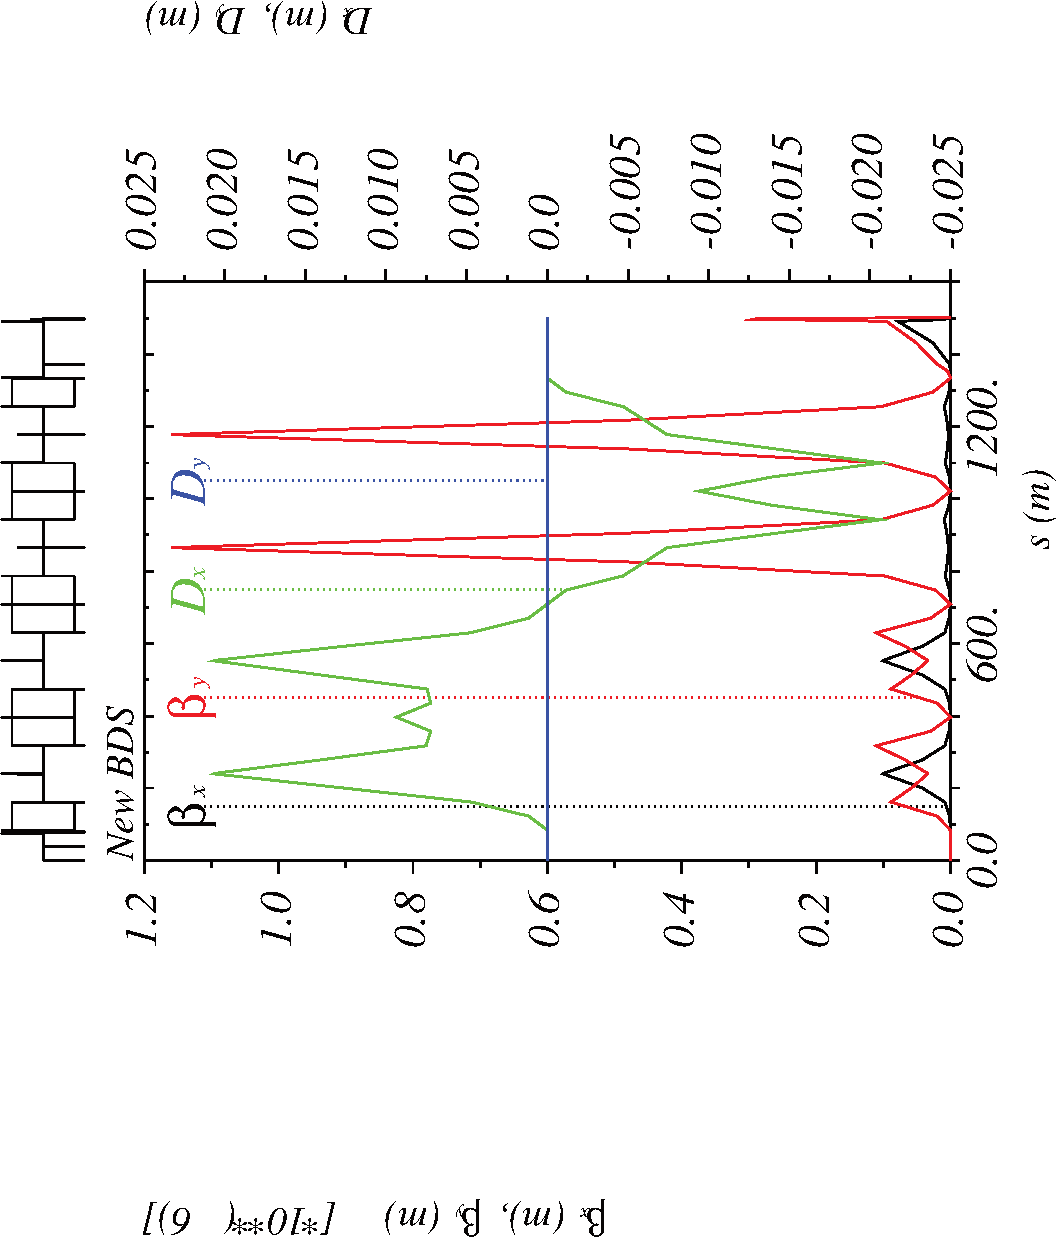
\includegraphics[scale=0.4,angle=-90]{CLICtrad_etax-crop.pdf}
 \end{textblock}
\end{frame}
\begin{frame}{CLIC 3TeV Non-local (trad)}
  \setlength{\TPHorizModule}{1pt}
  \setlength{\TPVertModule}{1pt}
 \begin{textblock}{400}(50,50)
 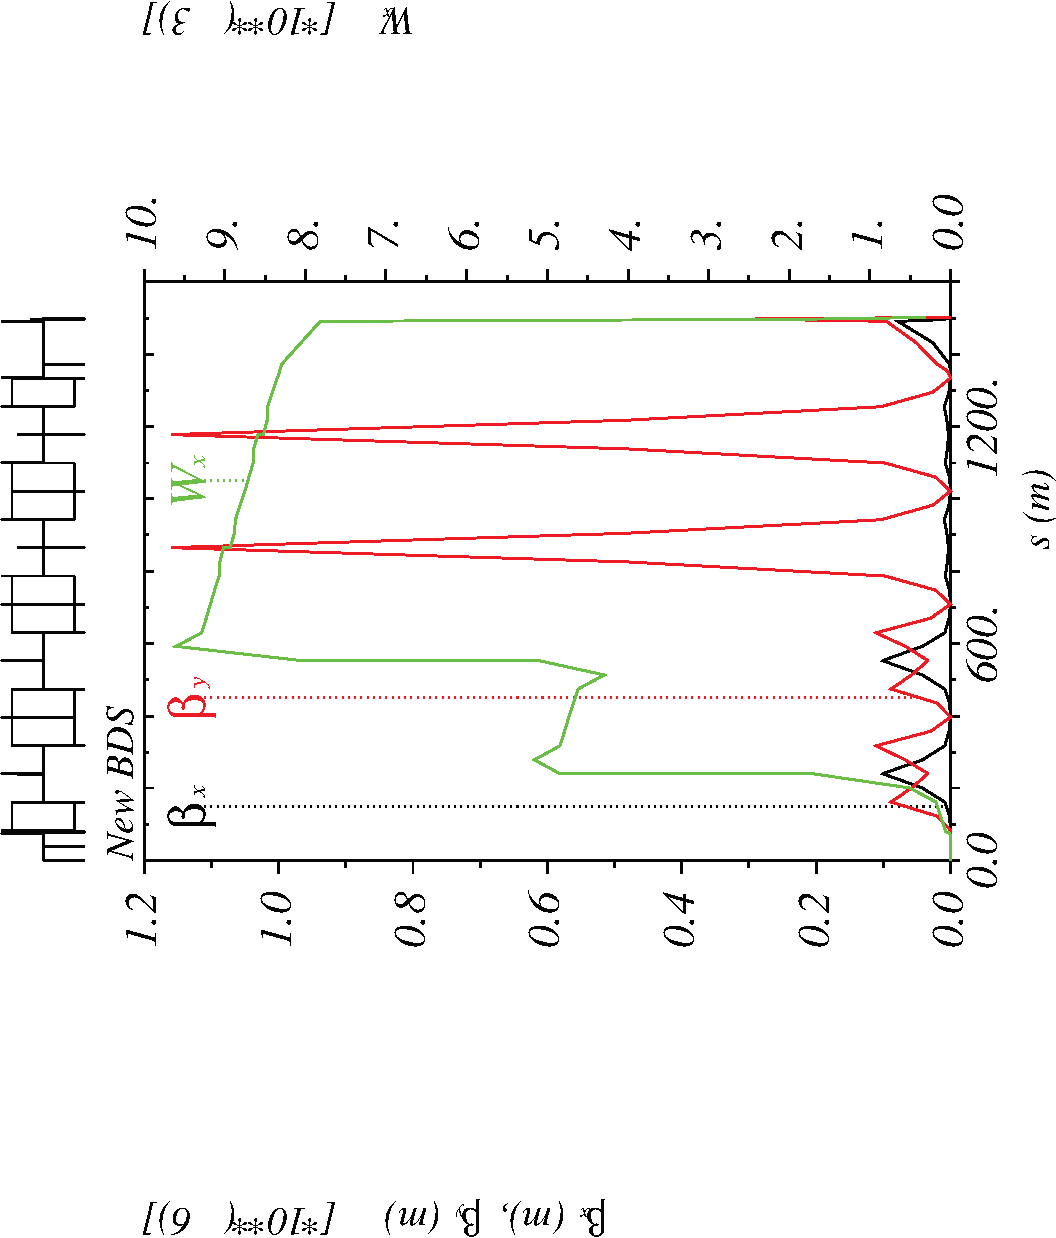
\includegraphics[scale=0.4,angle=-90]{CLICtrad_wx-crop.pdf}
 \end{textblock}
\end{frame}
\begin{frame}{CLIC 3TeV Non-local (trad)}
  \setlength{\TPHorizModule}{1pt}
  \setlength{\TPVertModule}{1pt}
 \begin{textblock}{400}(50,50)
 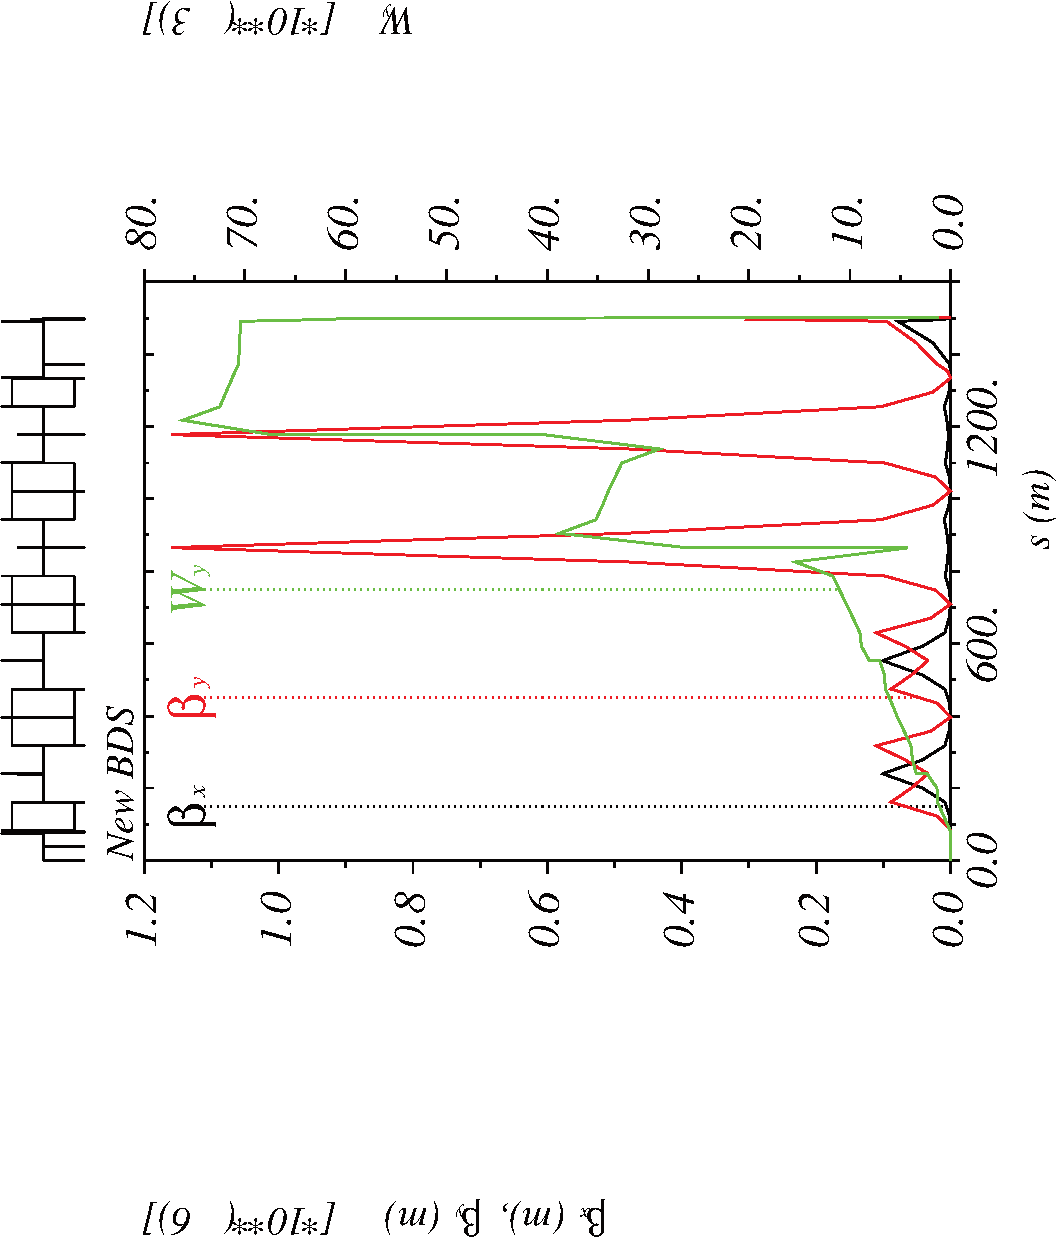
\includegraphics[scale=0.4,angle=-90]{CLICtrad_wy-crop.pdf}
 \end{textblock}
\end{frame}
\begin{frame}{CLIC 3TeV Non-local (trad)}
  \setlength{\TPHorizModule}{1pt}
  \setlength{\TPVertModule}{1pt}
 \begin{textblock}{400}(50,50)
 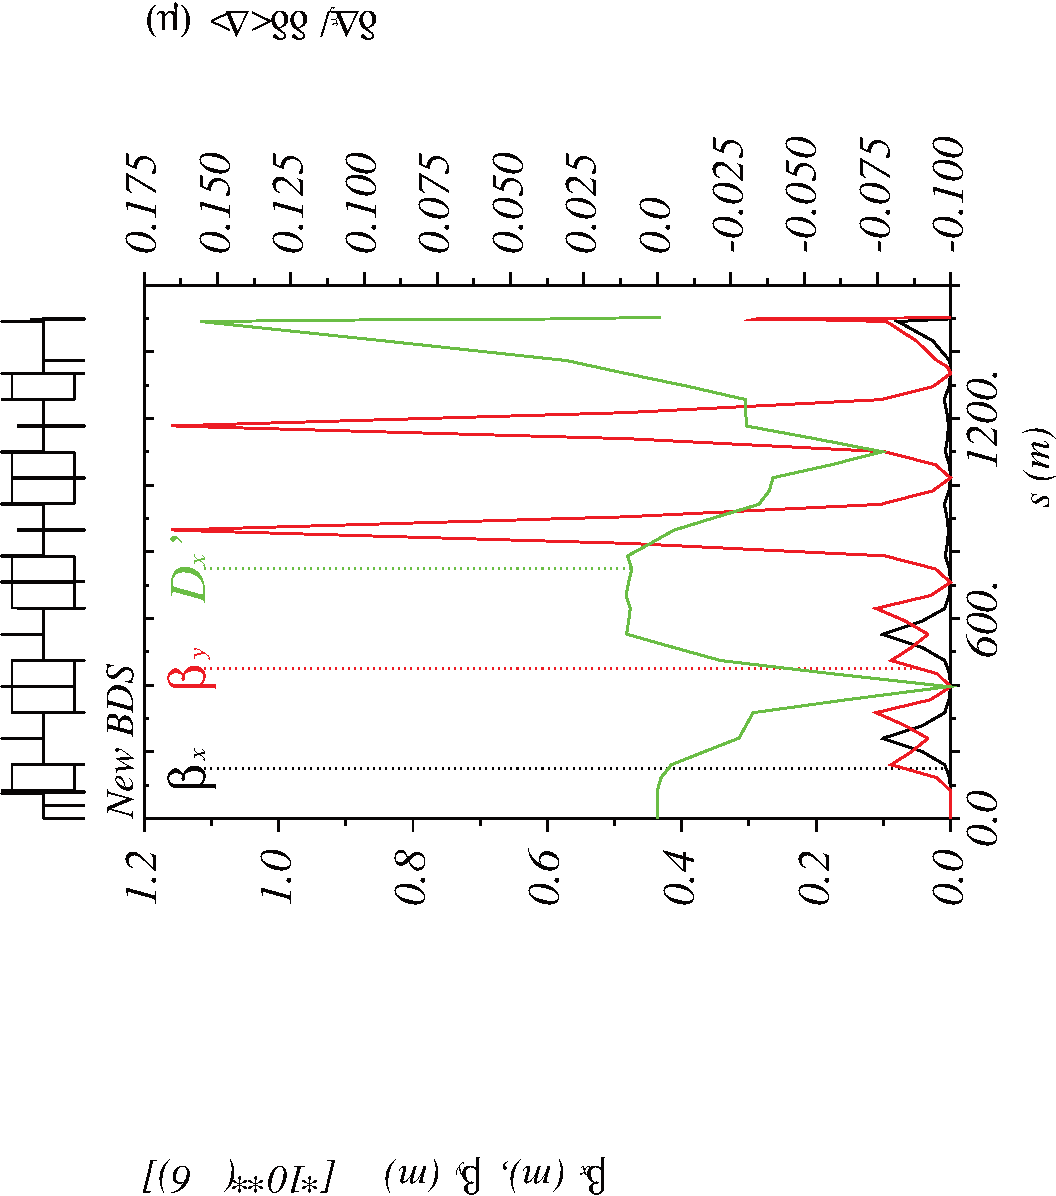
\includegraphics[scale=0.4,angle=-90]{CLICtrad_ddx-crop.pdf}
 \end{textblock}
\end{frame}
% \begin{frame}{CLIC 3TeV Non-local (trad)}
%   \setlength{\TPHorizModule}{1pt}
%   \setlength{\TPVertModule}{1pt}
%  \begin{textblock}{400}(50,50)
%  \includegraphics[scale=0.4,angle=-90]{CLICtrad_ddpx-crop.pdf}
%  \end{textblock}
% \end{frame}
\section{ILC 500 GeV}
\begin{frame}
 \color{blue}\Large ILC 500 GeV
\end{frame}
\begin{frame}{ILC 500 GeV (Local)}
  \setlength{\TPHorizModule}{1pt}
  \setlength{\TPVertModule}{1pt}
 \begin{textblock}{400}(50,50)
 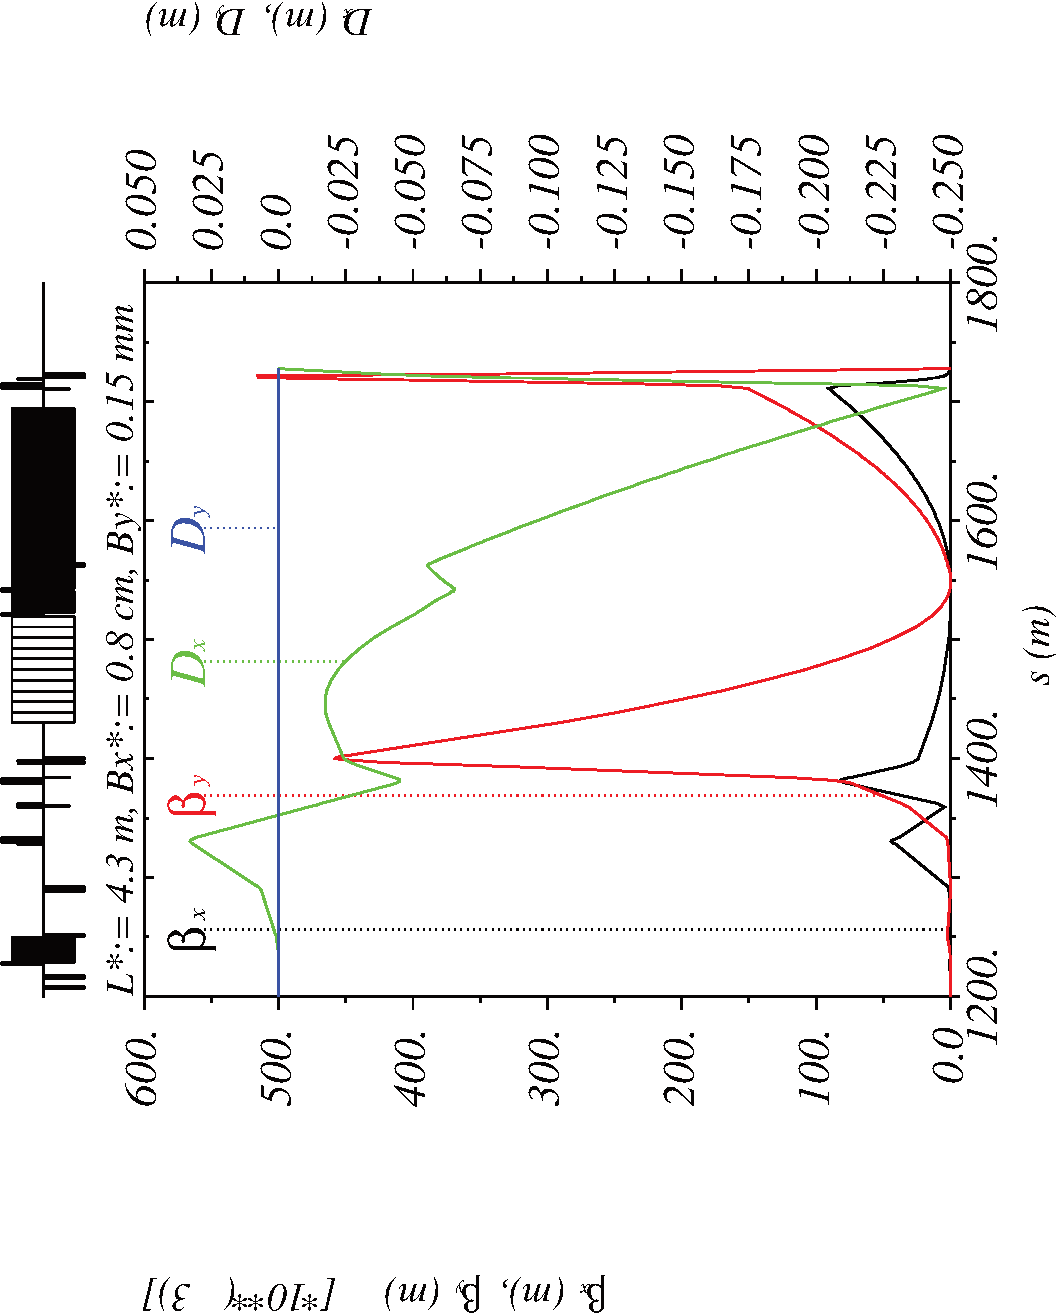
\includegraphics[scale=0.4,angle=-90]{ILClocal_etax-crop.pdf}
 \end{textblock}
\end{frame}
\begin{frame}{ILC 500 GeV (Local)}
  \setlength{\TPHorizModule}{1pt}
  \setlength{\TPVertModule}{1pt}
 \begin{textblock}{400}(50,50)
 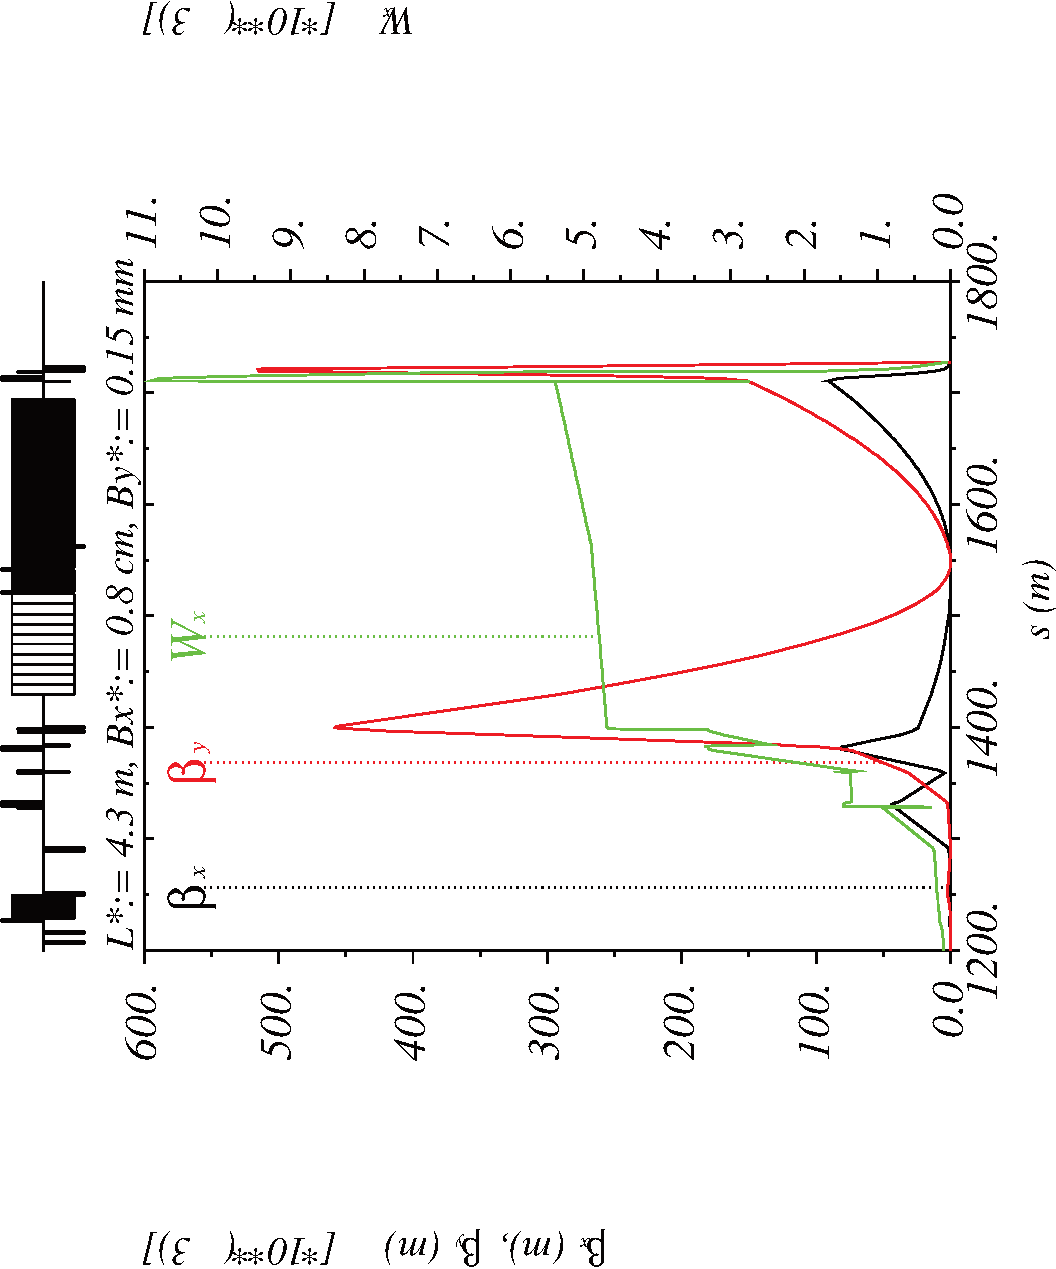
\includegraphics[scale=0.4,angle=-90]{ILClocal_wx-crop.pdf}
 \end{textblock}
\end{frame}
\begin{frame}{ILC 500 GeV (Local)}
  \setlength{\TPHorizModule}{1pt}
  \setlength{\TPVertModule}{1pt}
 \begin{textblock}{400}(50,50)
 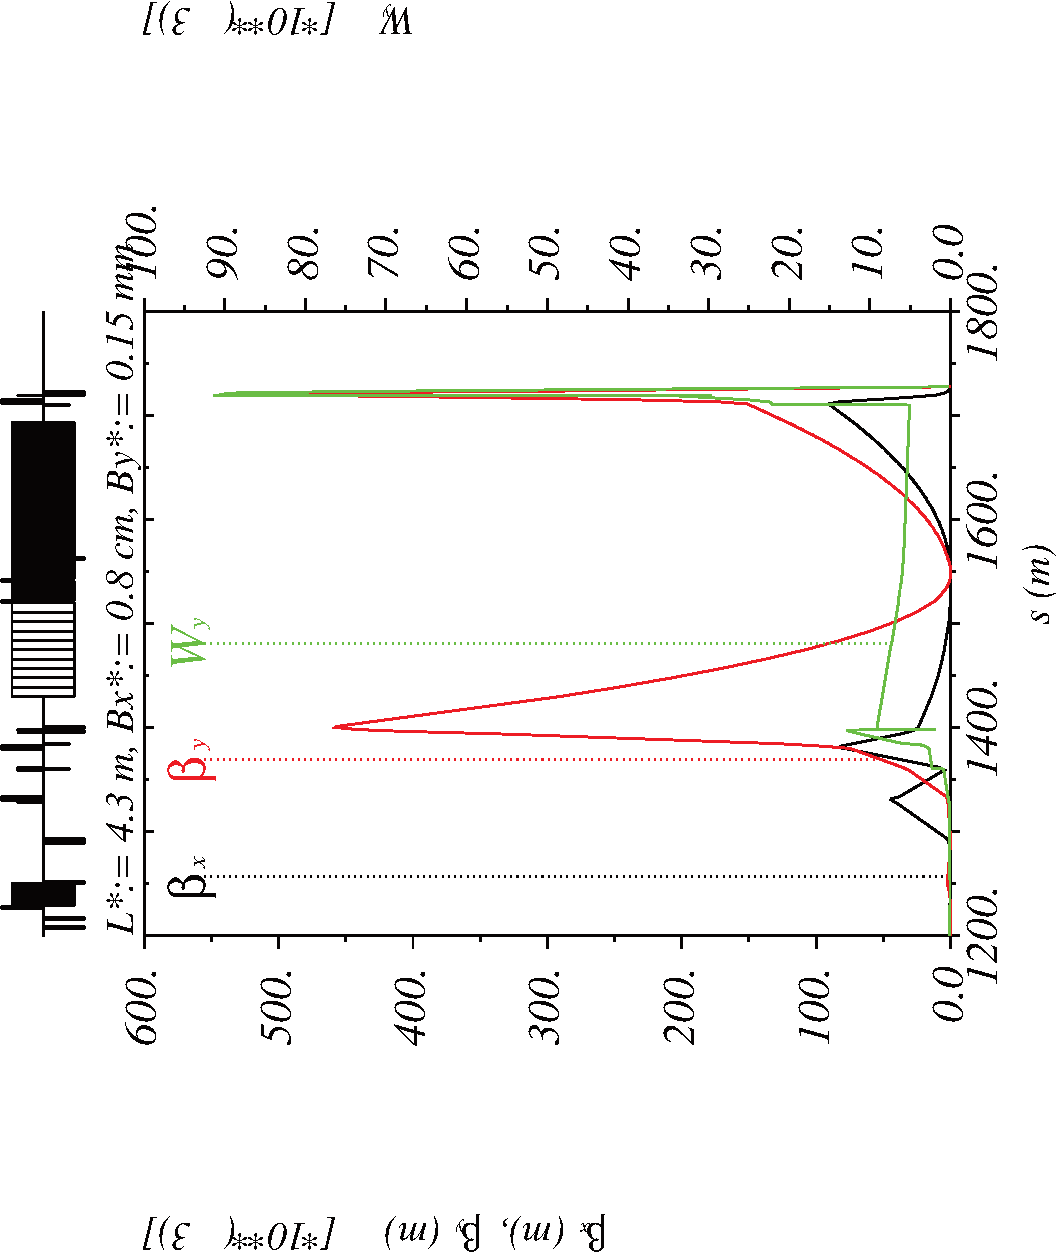
\includegraphics[scale=0.4,angle=-90]{ILClocal_wy-crop.pdf}
 \end{textblock}
\end{frame}
\begin{frame}{ILC 500 GeV (Local)}
  \setlength{\TPHorizModule}{1pt}
  \setlength{\TPVertModule}{1pt}
 \begin{textblock}{400}(50,50)
 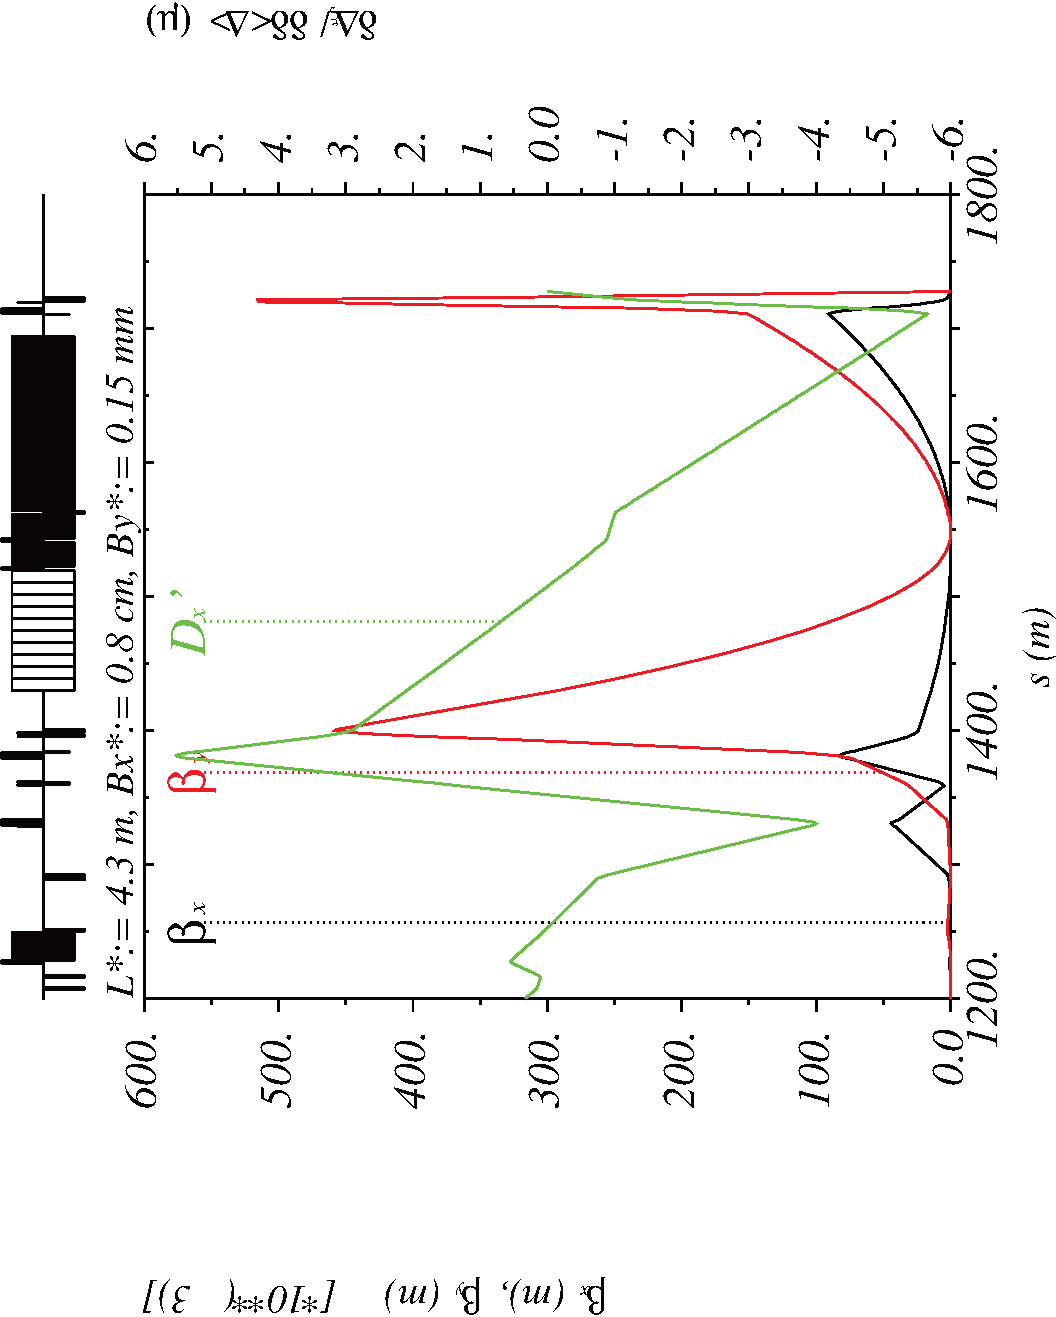
\includegraphics[scale=0.4,angle=-90]{ILClocal_ddx-crop.pdf}
 \end{textblock}
\end{frame}

\section{CLIC 500GeV Non-interleaved Lattice}
\begin{frame}
 \color{blue}\Large CLIC 500 GeV Non-interleaved Lattice
\end{frame}
\begin{frame}{Current 500 GeV Lattice Parameters (from CDR)}
\begin{center}
 \begin{tabular}{|l|c|}\hline\hline
  \textbf{Parameter [Units]} & \textbf{Value}\\\hline
  Length (linac exit to IP distance/side [m]) & 1750\\
  Maximum energy/beam [TeV] & 0.25\\
  Distance from IP to first quad, $L^*$ [m] & 4.3\\
  Crossing angle at the IP [mrad] & 18.6\\
  Nominal core beam size at IP, $\sigma^*$, $x/y$ [nm] & 202/2.3\\
  Nominal beam divergence at IP, $\theta^*$, $x/y$ [$\mu$rad] & 25/23\\
  Nominal beta-function at IP, $\beta^*$, $x/y$ [mm] & 8/0.1\\
  Nominal bunch length, $\sigma_z$ [$\mu$m] & 72\\
  Nominal disruption parameters, $D$, $x/y$ & 0.1/12\\
  Nominal bunch population, $N$ & $6.8\times10^9$\\
  Beam power in each beam [MW] & 4.9\\
  Preferred entrance train to train jitter [$\sigma$] & $<0.2$\\
  Typical nominal collimation aperture, $x/y$ [$\sigma_x/\sigma_y$] & 10/55\\
  Vacuum pressure level, near/far from IP [$10^{-9}$ mbar] & 100/10\\\hline
 \end{tabular}
 \end{center}
\end{frame}
\begin{frame}{CLIC 500GeV Non-interleaved Lattice}
  \setlength{\TPHorizModule}{1pt}
  \setlength{\TPVertModule}{1pt}
 \begin{textblock}{400}(50,50)
 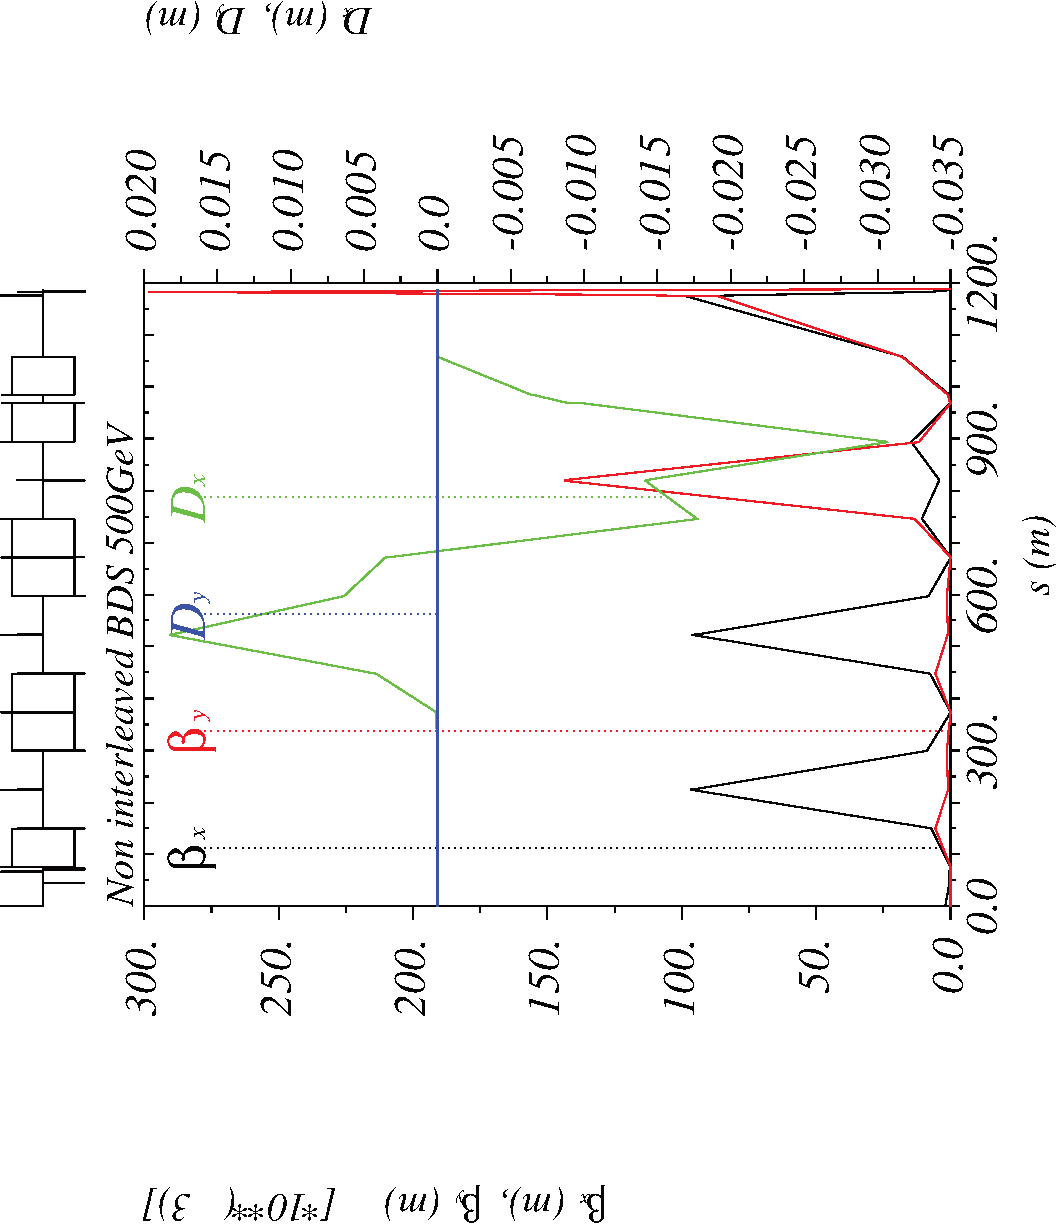
\includegraphics[scale=0.4,angle=-90]{CLIC500noninter_etax-crop.pdf}
 \end{textblock}
\end{frame}
\begin{frame}{CLIC 500GeV Non-interleaved Lattice}
  \setlength{\TPHorizModule}{1pt}
  \setlength{\TPVertModule}{1pt}
 \begin{textblock}{400}(50,50)
 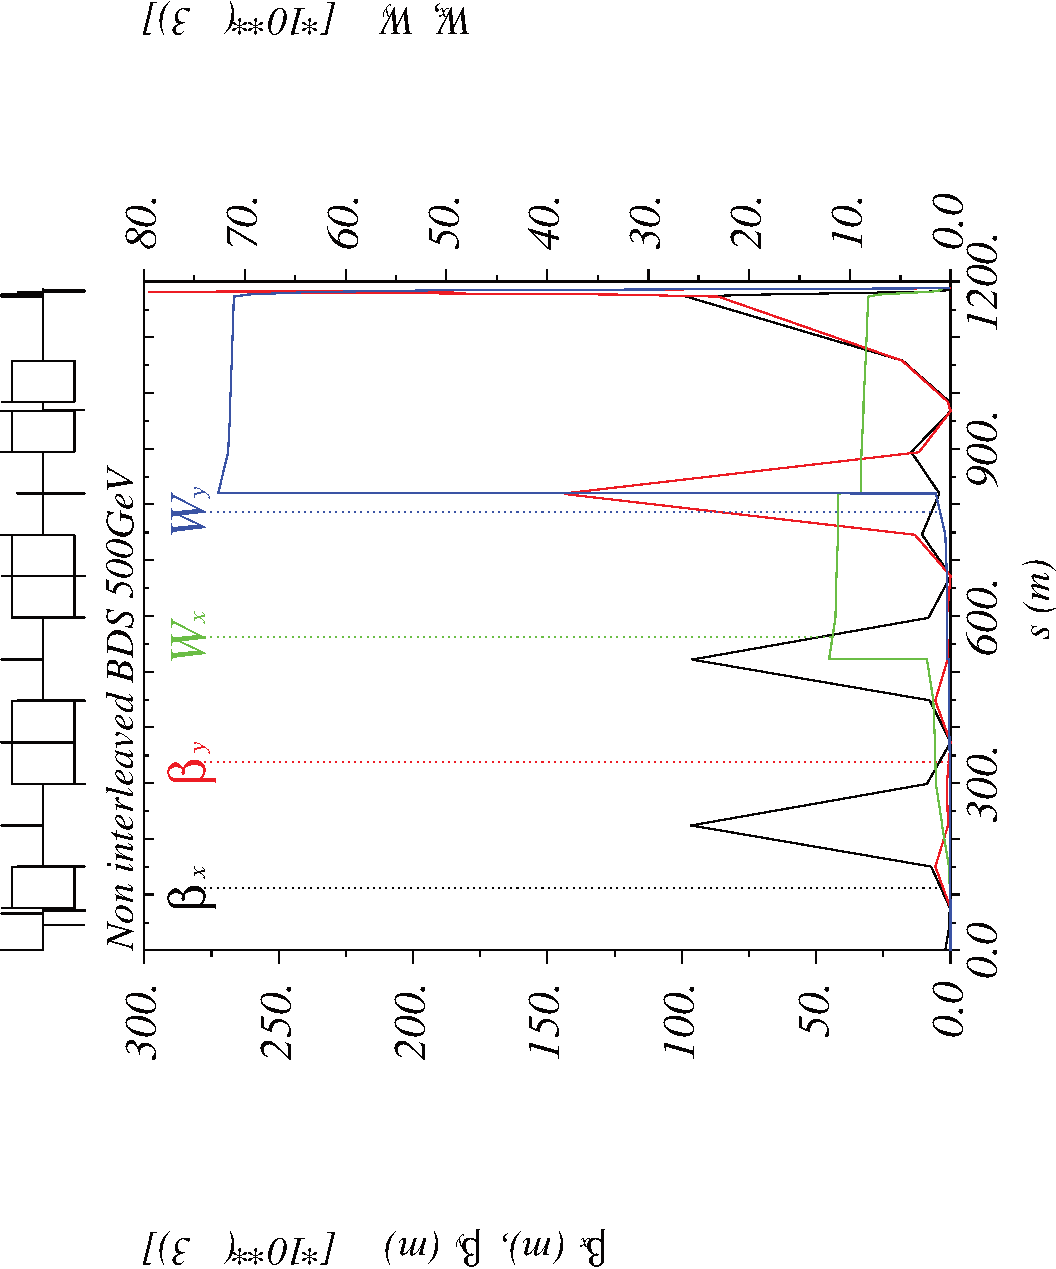
\includegraphics[scale=0.4,angle=-90]{CLIC500noninter_wxwy-crop.pdf}
 \end{textblock}
\end{frame}
\begin{frame}{CLIC 500GeV Non-interleaved Lattice}
  \setlength{\TPHorizModule}{1pt}
  \setlength{\TPVertModule}{1pt}
 \begin{textblock}{400}(50,50)
 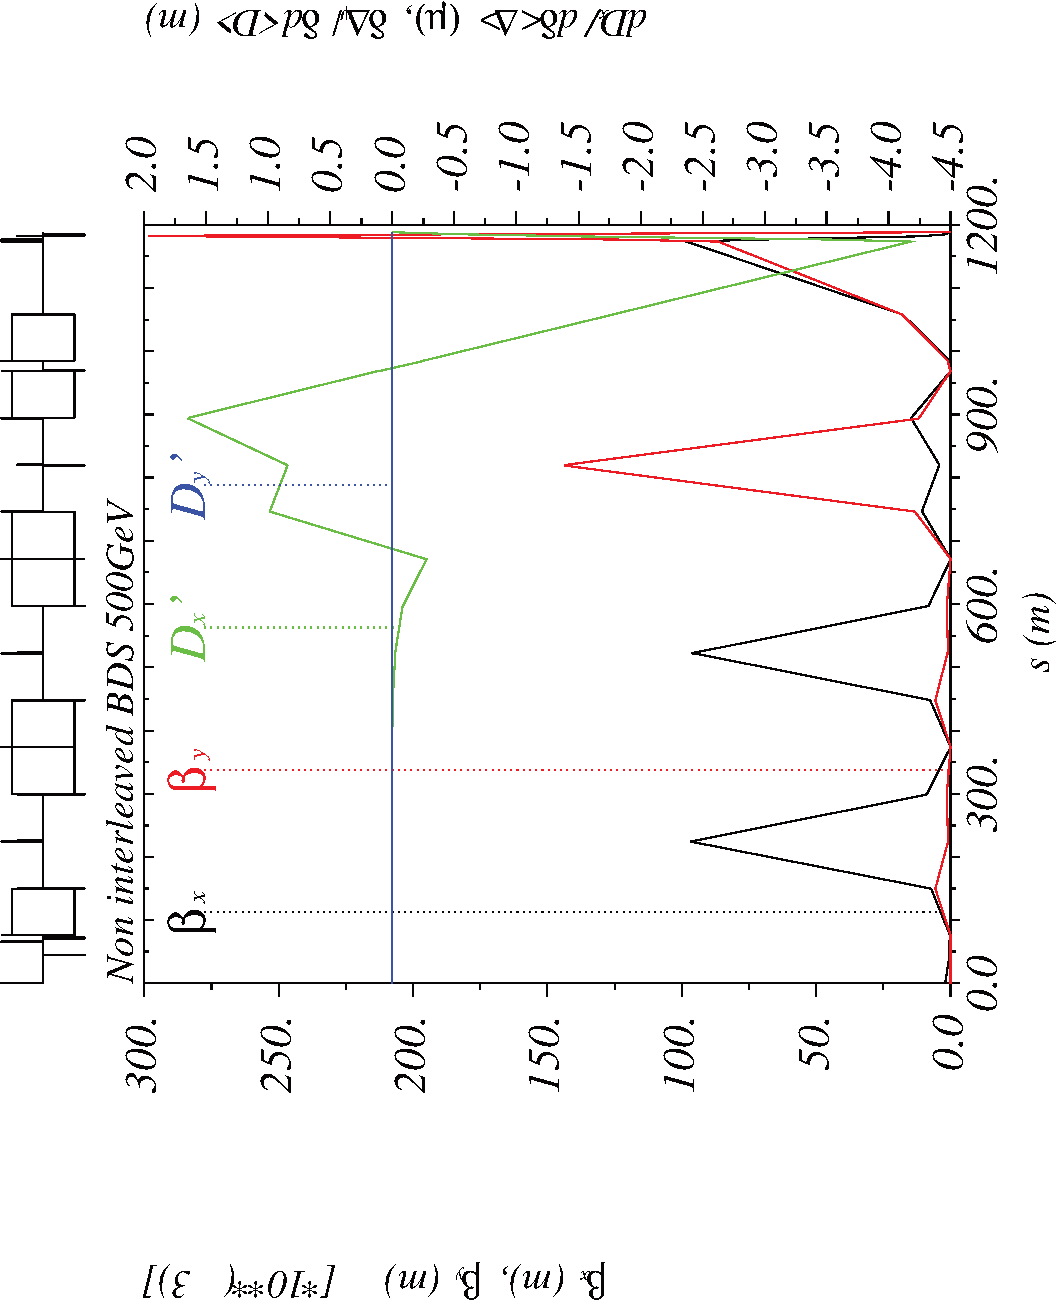
\includegraphics[scale=0.4,angle=-90]{CLIC500noninter_ddx-crop.pdf}
 \end{textblock}
\end{frame}
% \begin{frame}{Non-interleaved CLIC 500 GeV}%{Final Doublet (FD)}
%  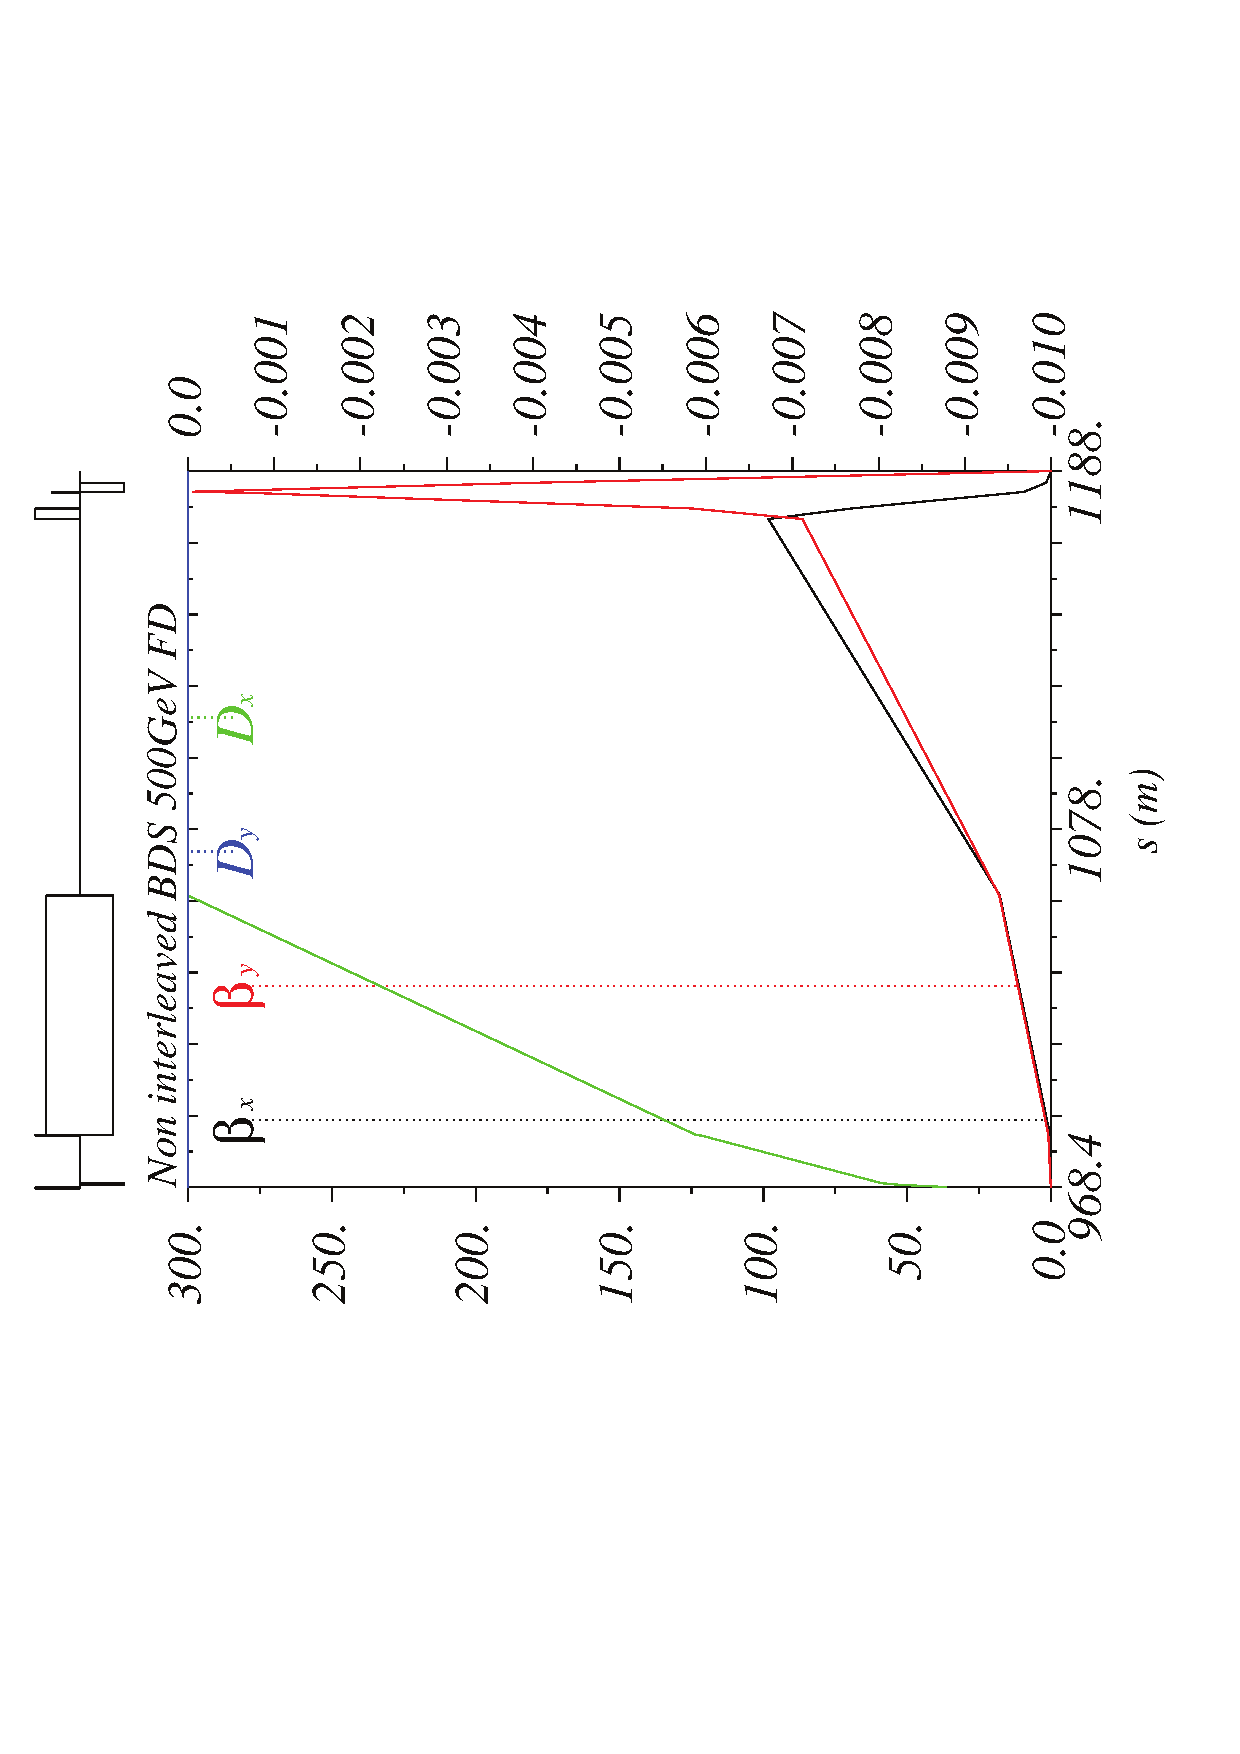
\includegraphics[scale=0.20,angle=-90]{madx001.pdf}
% % \end{frame}
% % \begin{frame}{Vertical Chromaticity Correction}
%  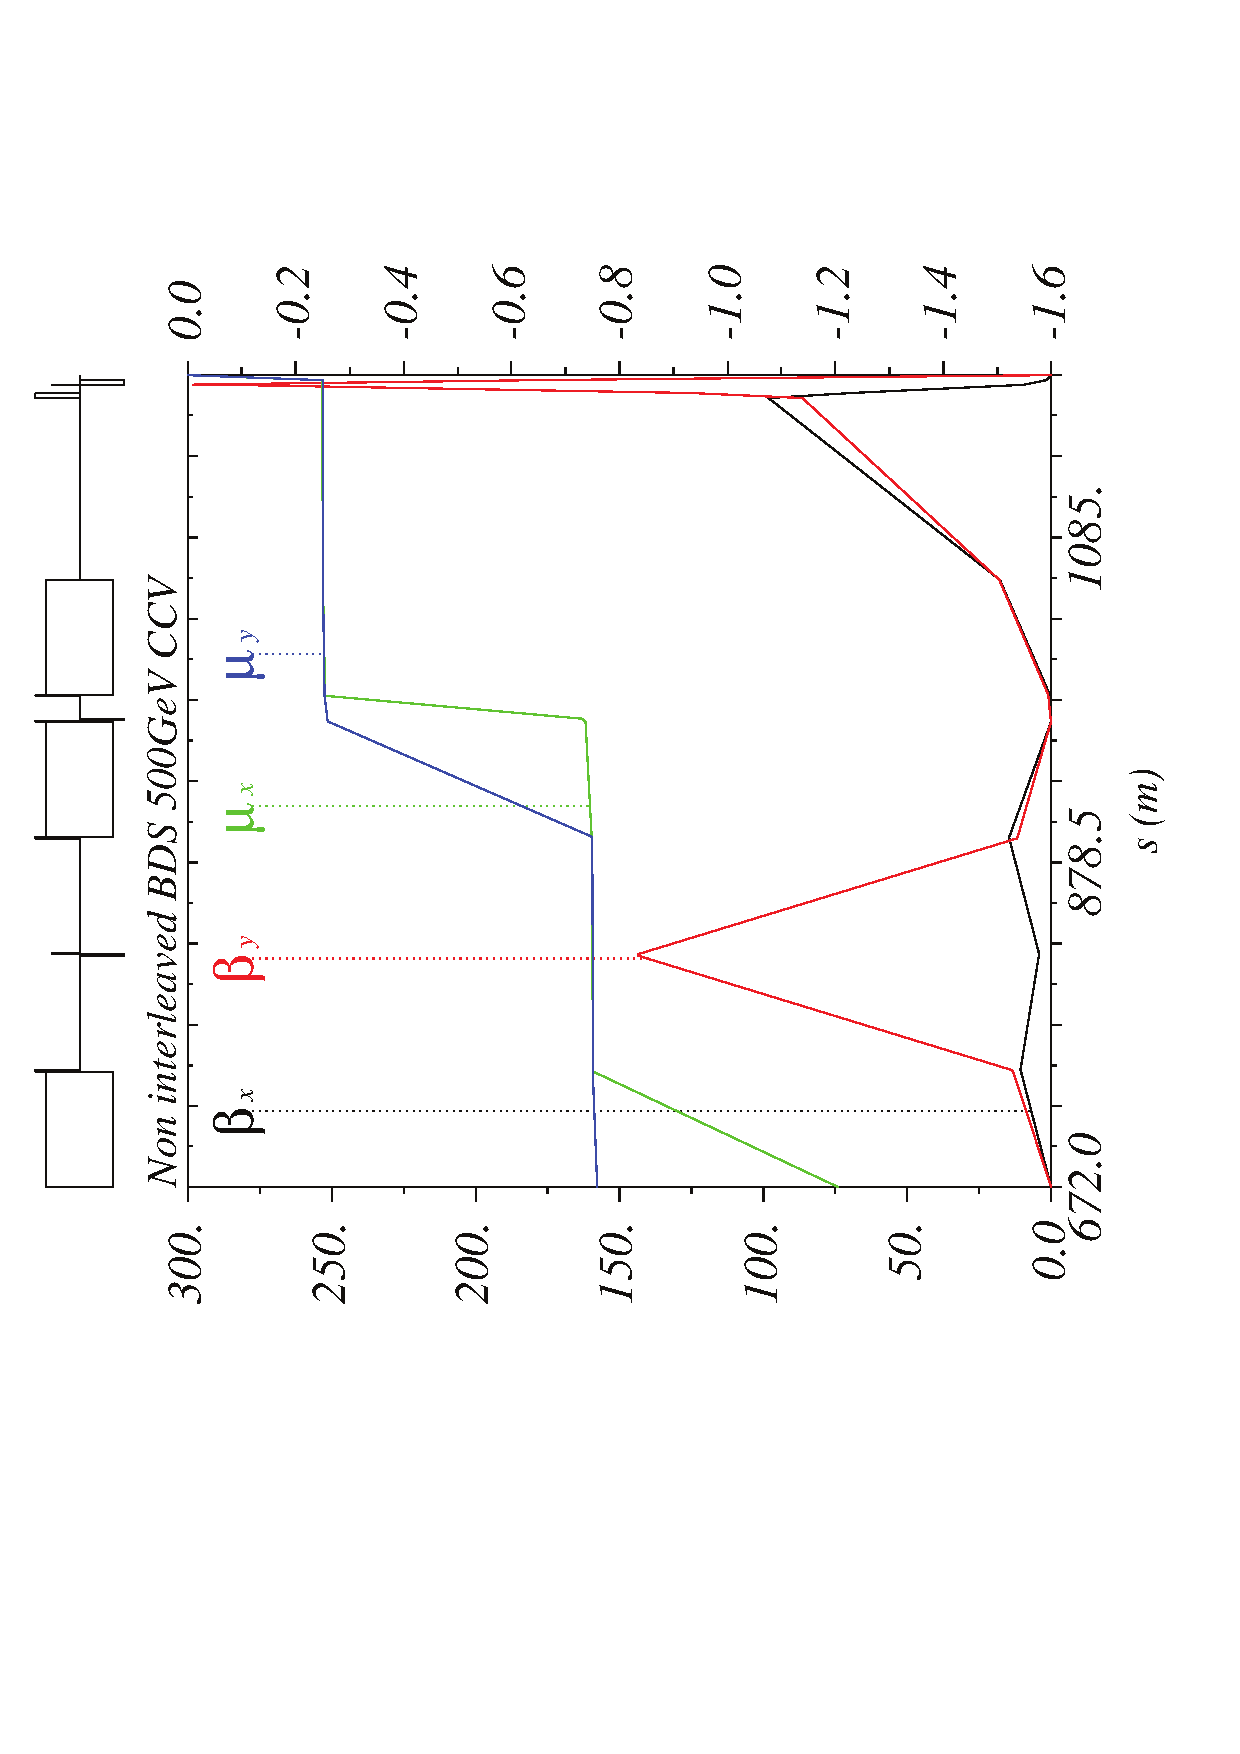
\includegraphics[scale=0.20,angle=-90]{madx002.pdf}\\
% % \end{frame}
% % \begin{frame}{Horizontal Chromaticity Correction}
%  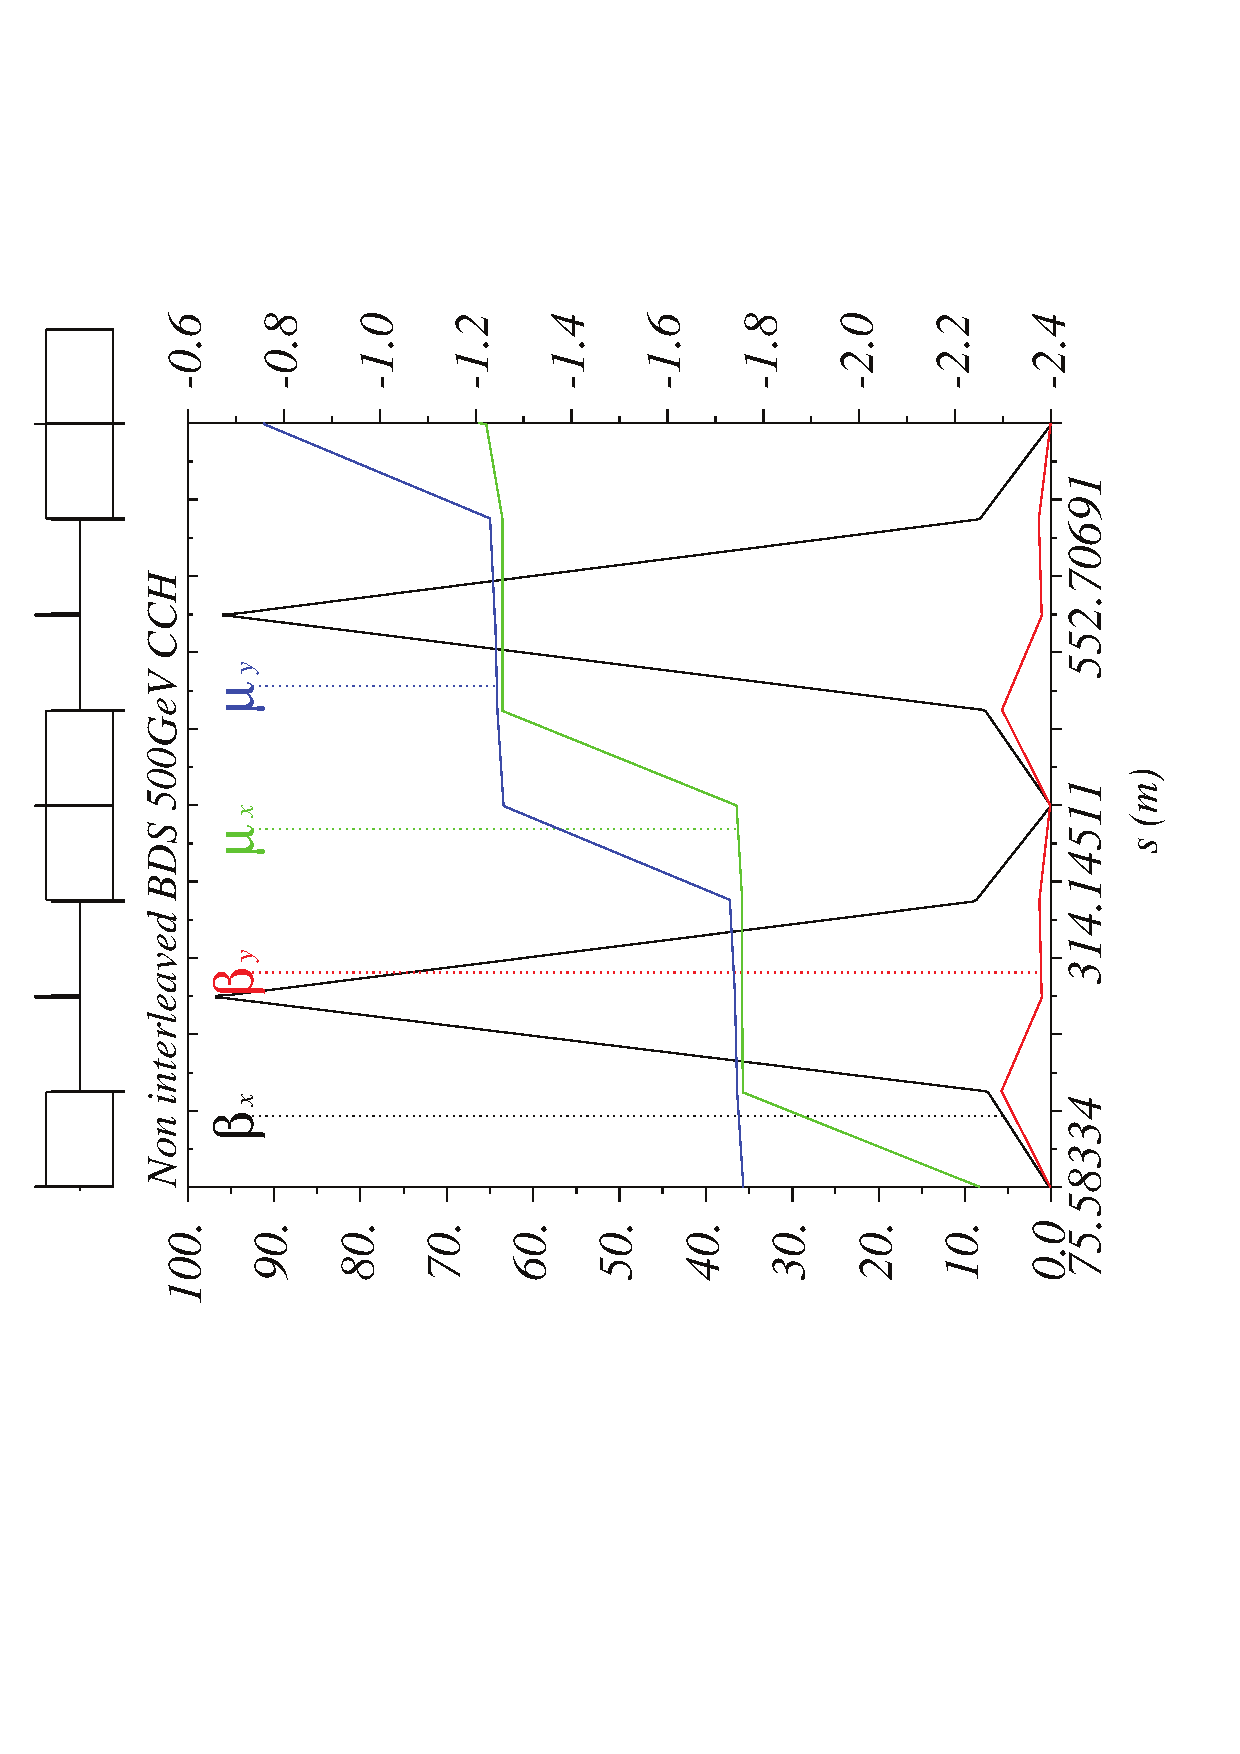
\includegraphics[scale=0.20,angle=-90]{madx003.pdf}
% % \end{frame}
% % \begin{frame}{The 500 GeV Non-interleaved Lattice}
%  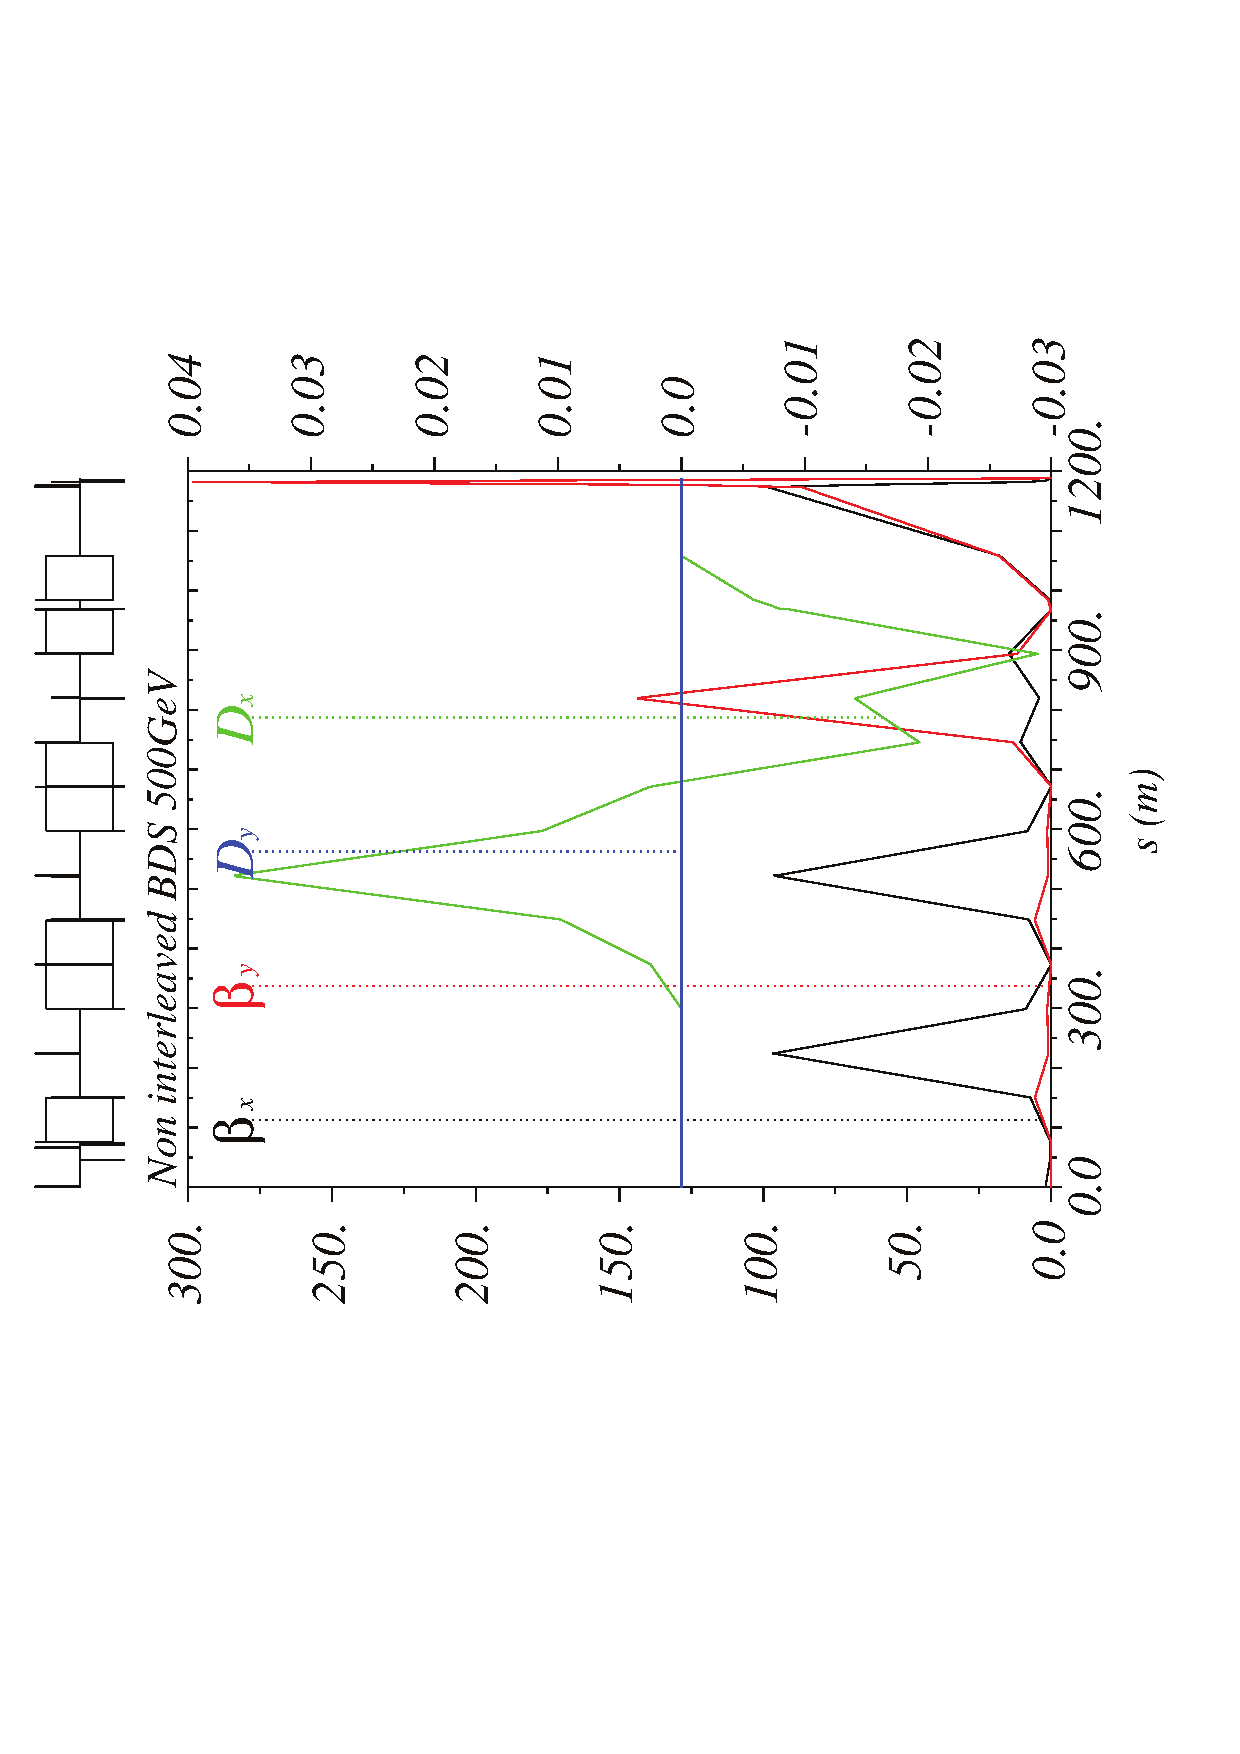
\includegraphics[scale=0.20,angle=-90]{madx005.pdf}
% \end{frame}
% \begin{frame}{Non-interleaved CLIC 500 GeV}%{Final Doublet (FD)}
%  \setlength{\TPHorizModule}{1pt}
%   \setlength{\TPVertModule}{1pt}
%   \begin{textblock}{400}(10,20)
%  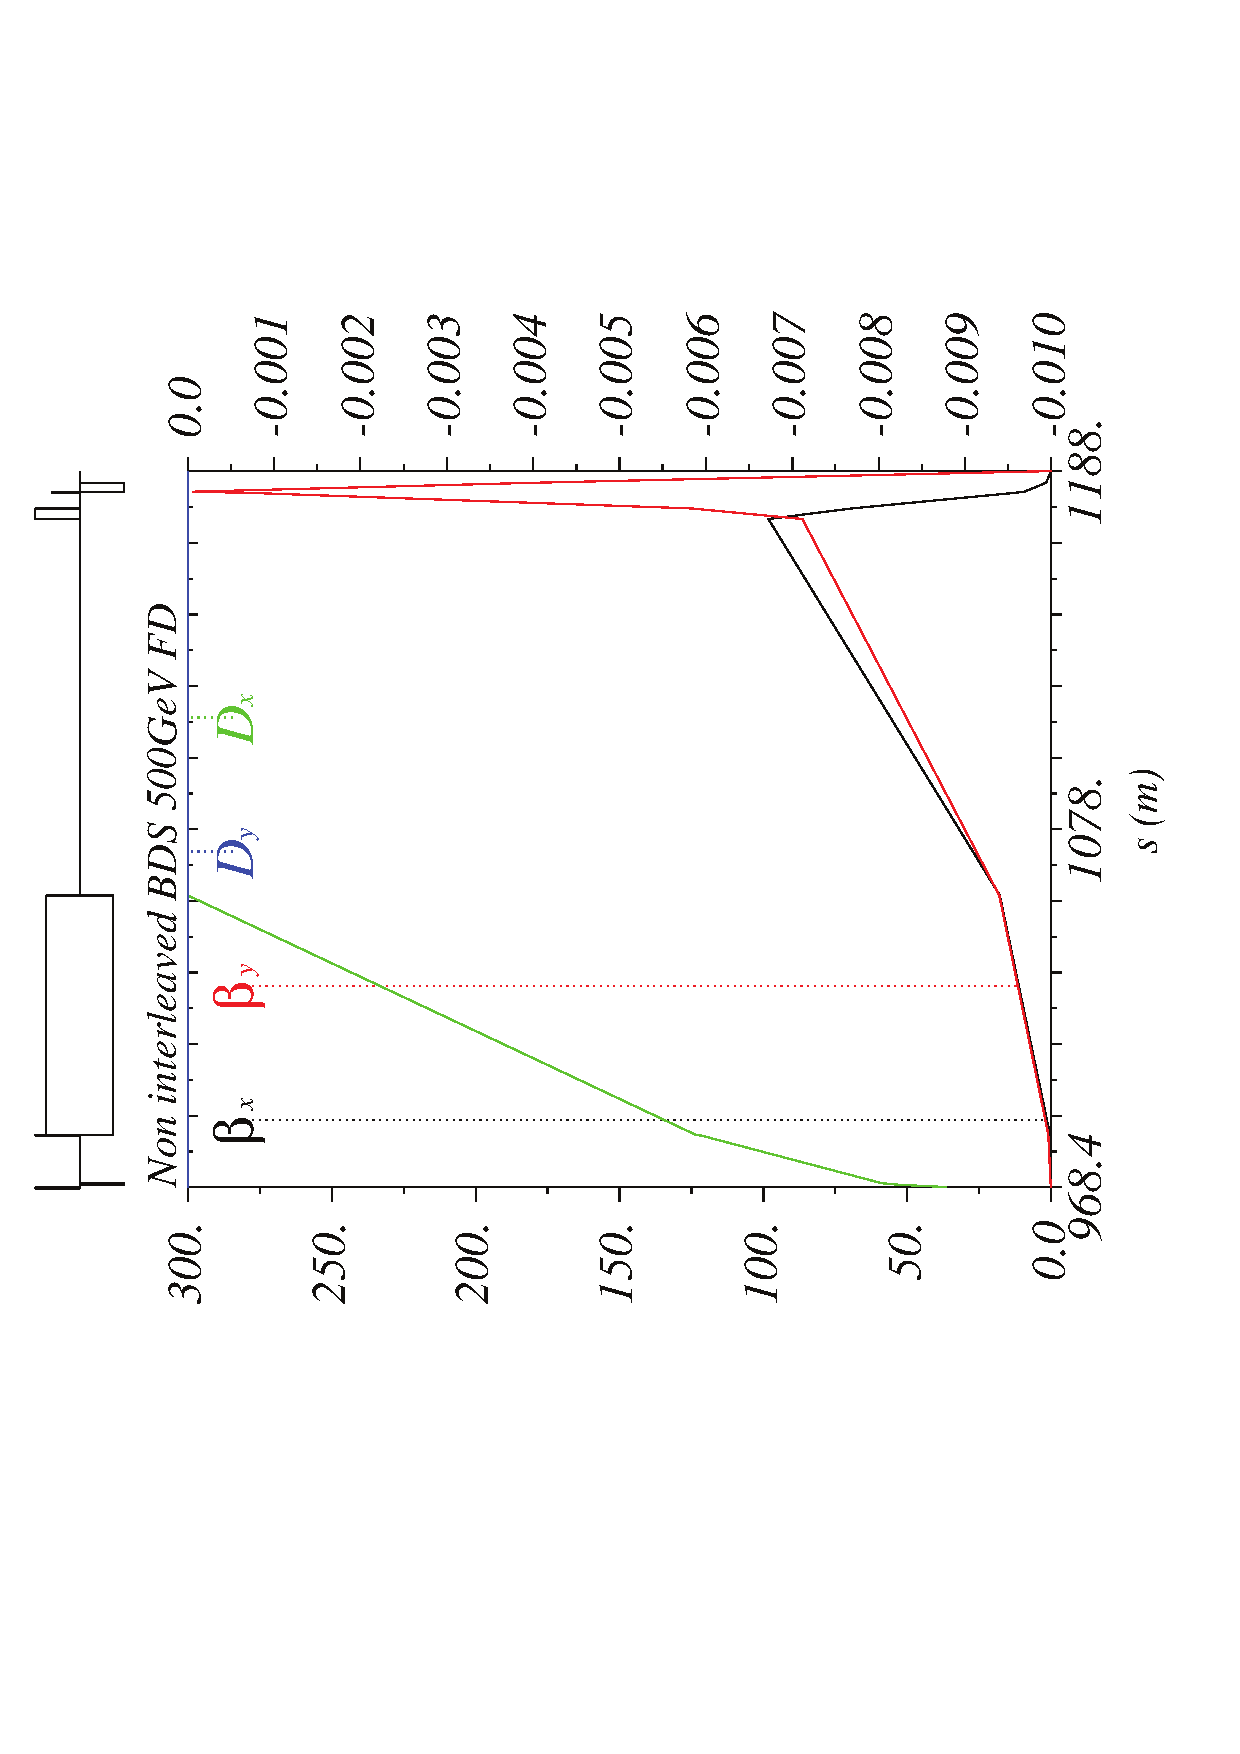
\includegraphics[scale=0.15,angle=-90]{madx001.pdf}
%  \end{textblock}
%  \begin{textblock}{400}(10,102)
%  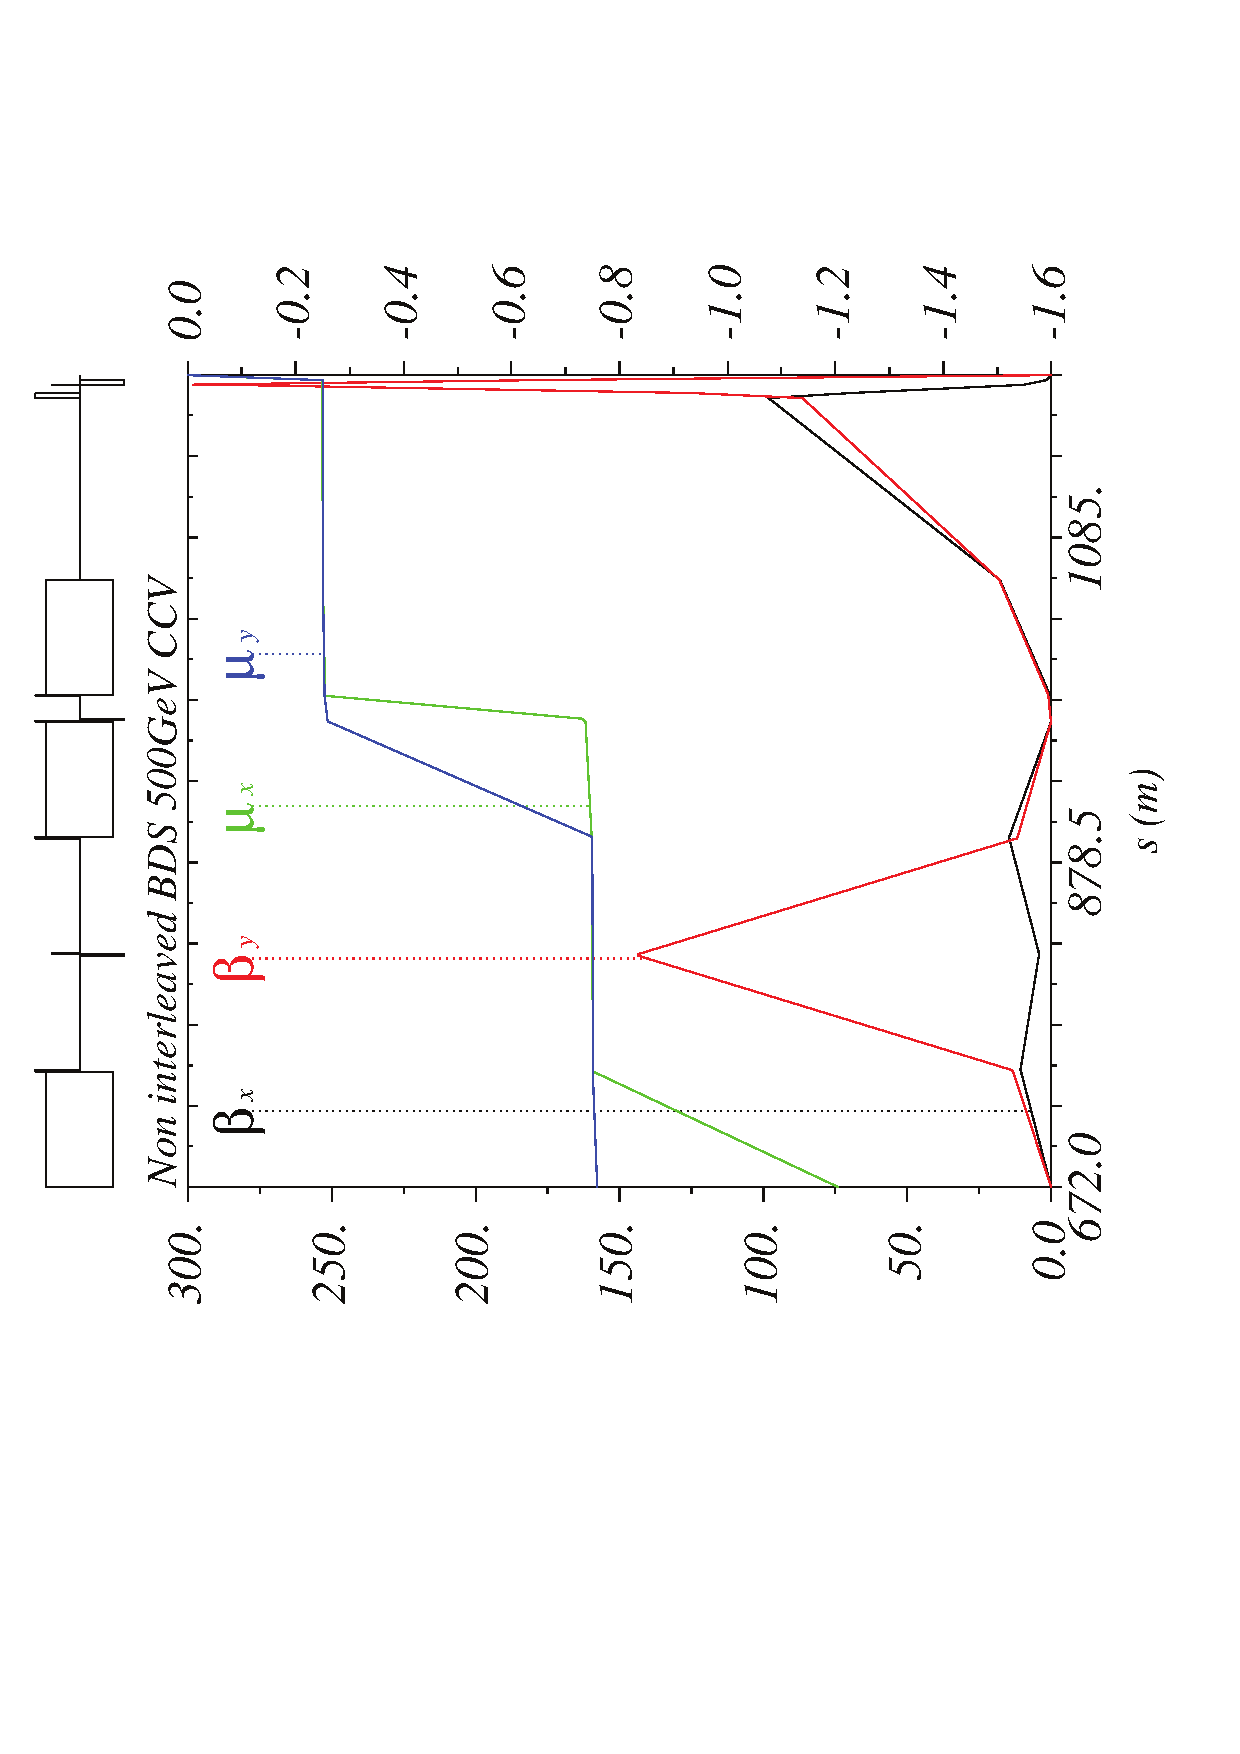
\includegraphics[scale=0.15,angle=-90]{madx002.pdf}
%  \end{textblock}
%  \begin{textblock}{400}(10,186)
%  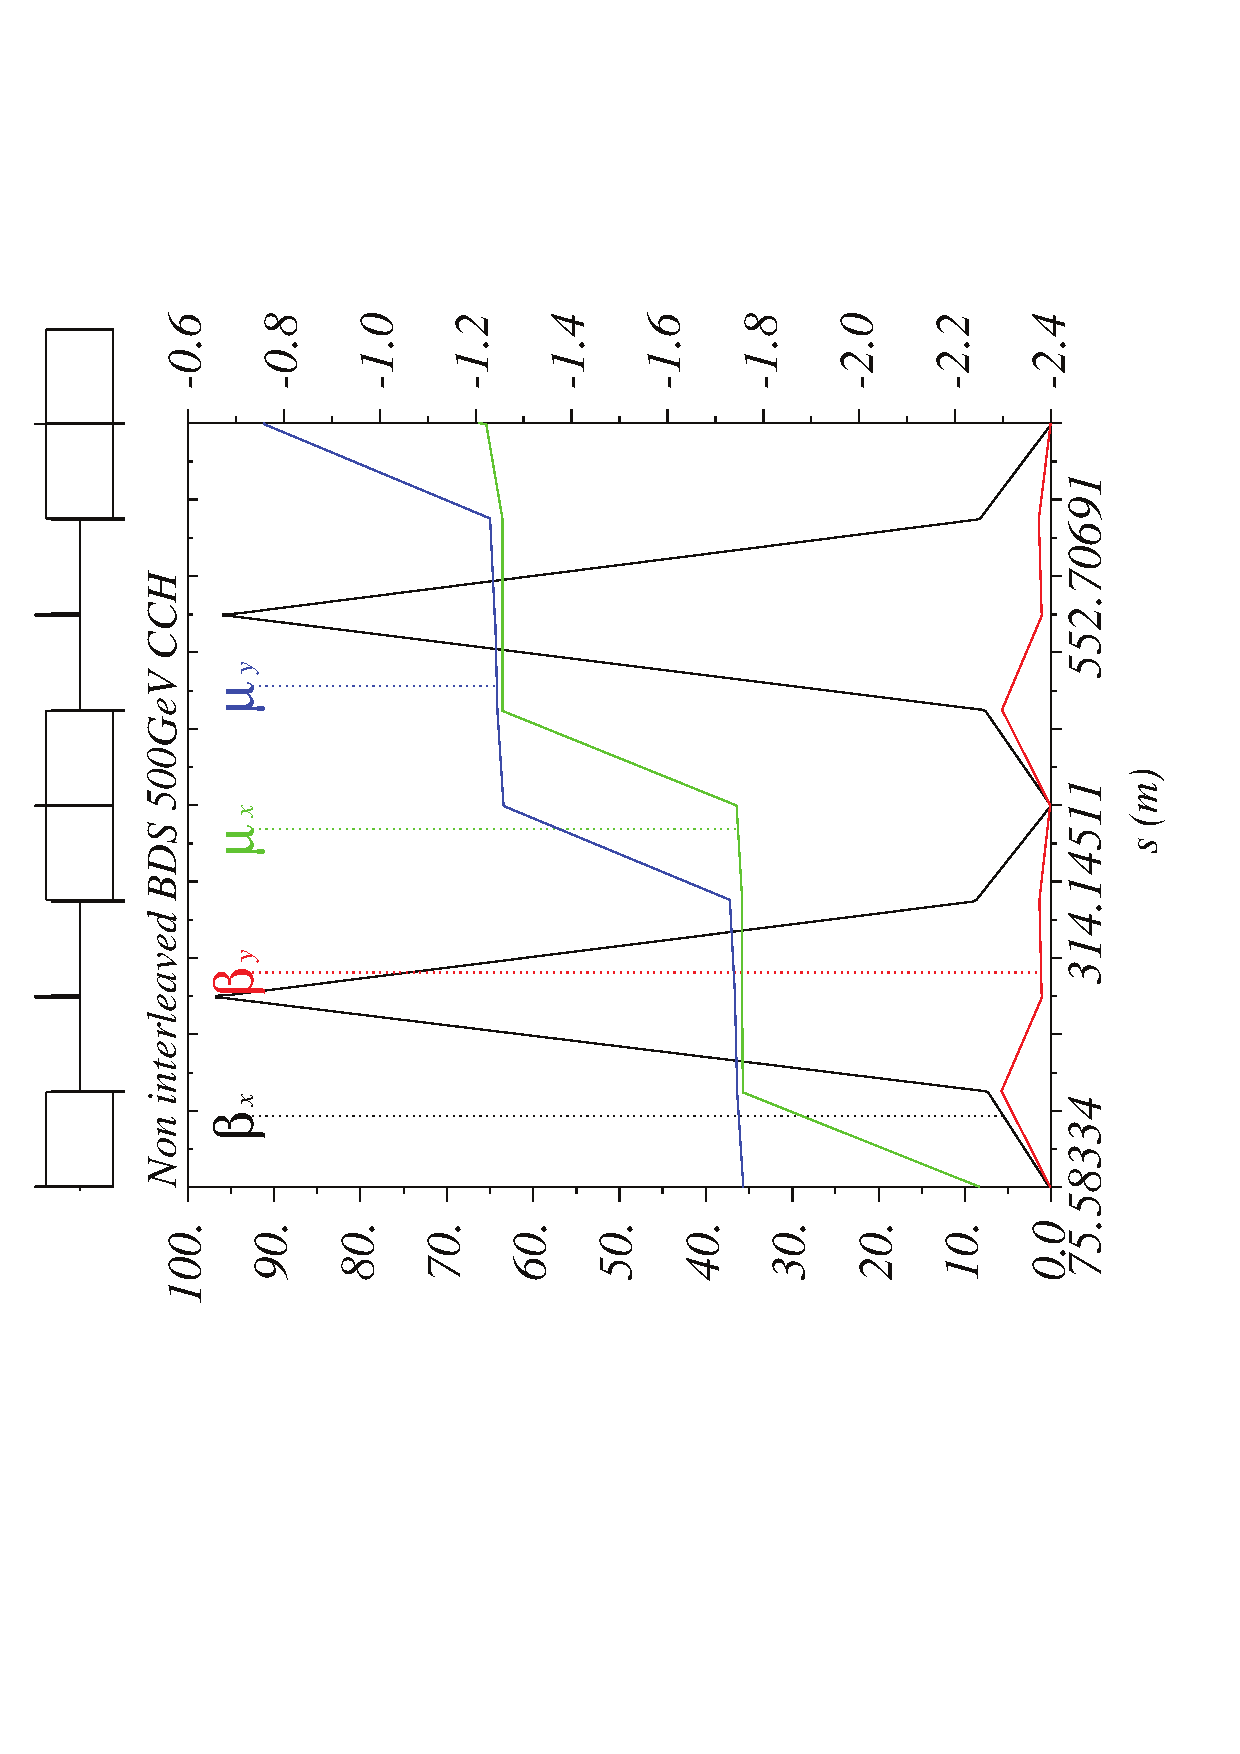
\includegraphics[scale=0.15,angle=-90]{madx003.pdf}
%  \end{textblock}
%  \begin{textblock}{400}(50,20)
%  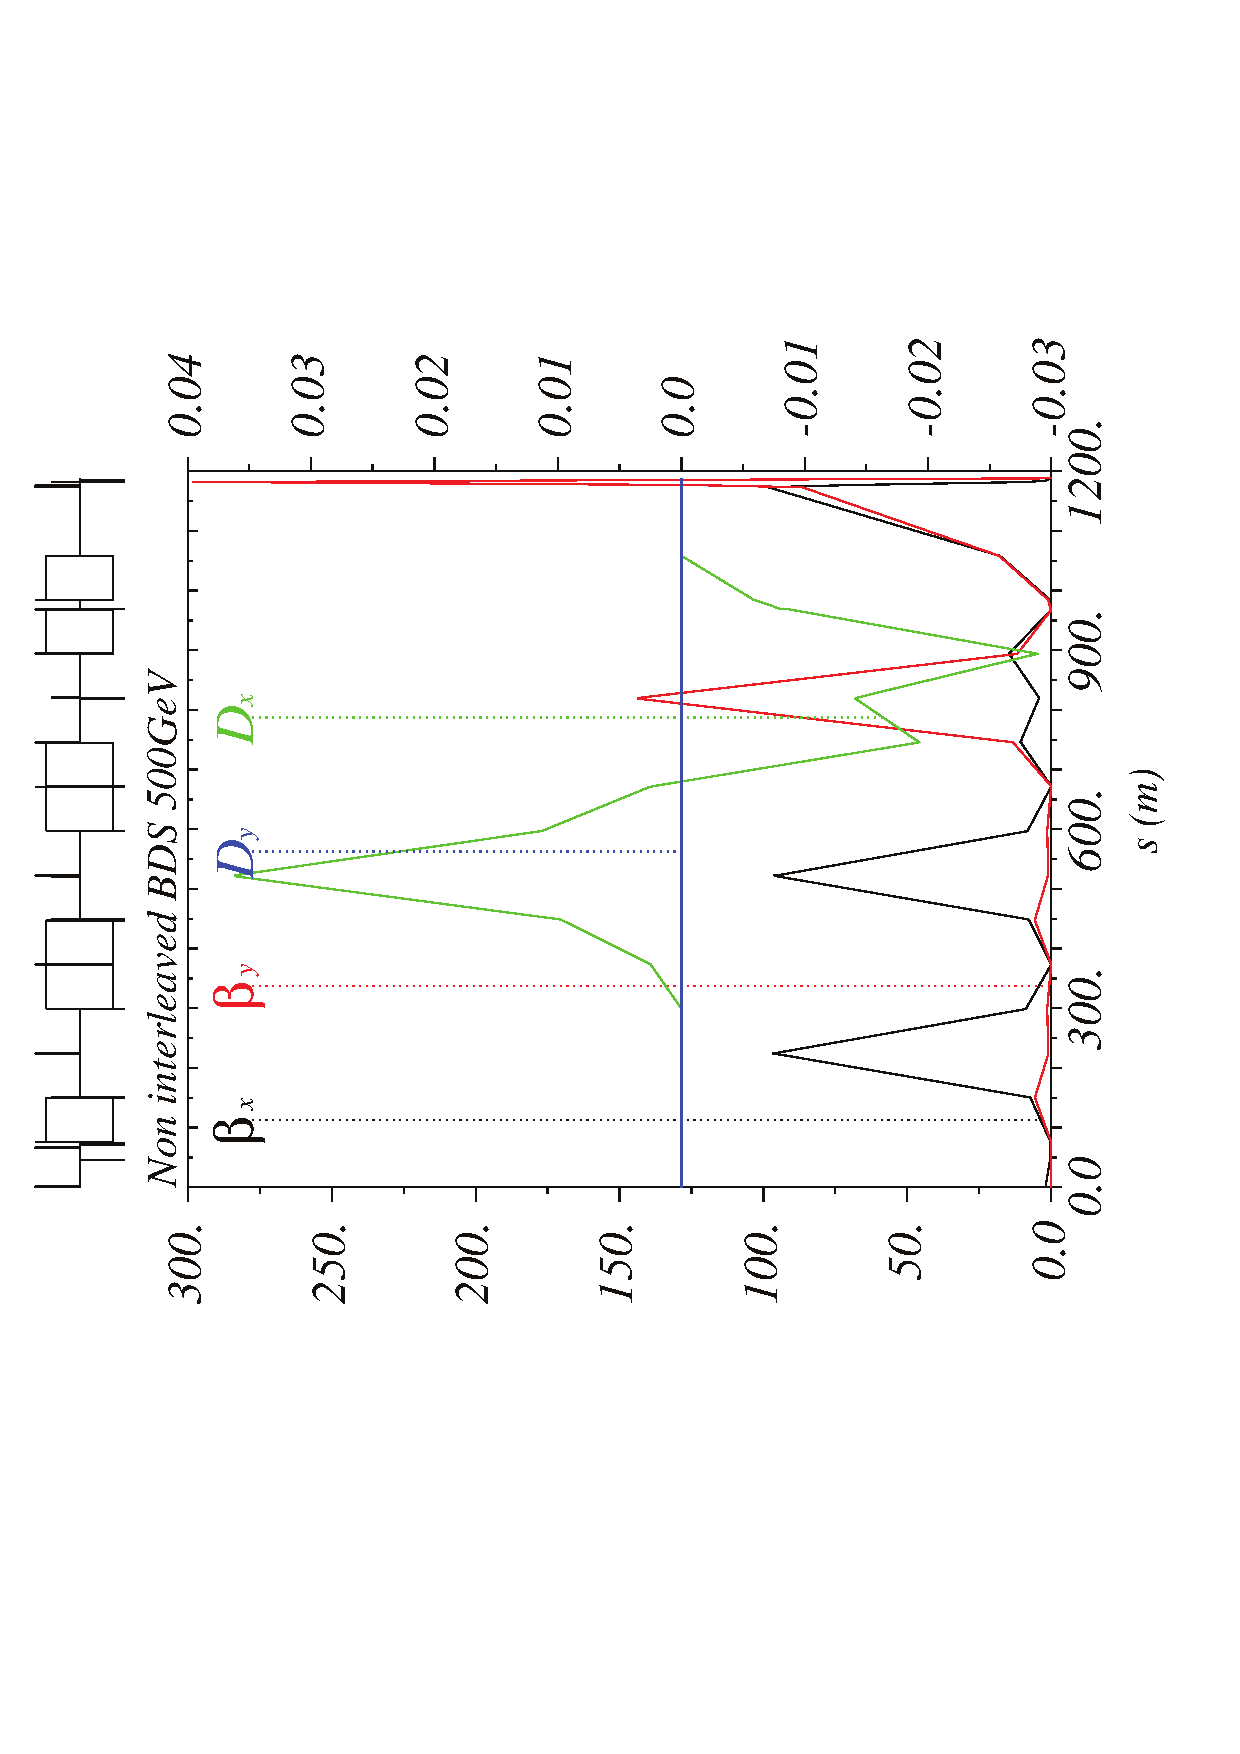
\includegraphics[scale=0.44,angle=-90]{madx005.pdf}
%  \end{textblock}
% \end{frame}
\begin{frame}{Non-interleaved CLIC 500 GeV (cont.)}
The lattice desing gives linear (order=1) beam size of :\par $\sigma_x = 1.9 \text{nm}$, $\sigma_y = 186 \text{nm}$\par
\vspace*{4cm}
$\sigma_{bends}=0.2$nm\par
\setlength{\TPHorizModule}{1pt}
  \setlength{\TPVertModule}{1pt}
 \begin{textblock}{400}(80,50)
 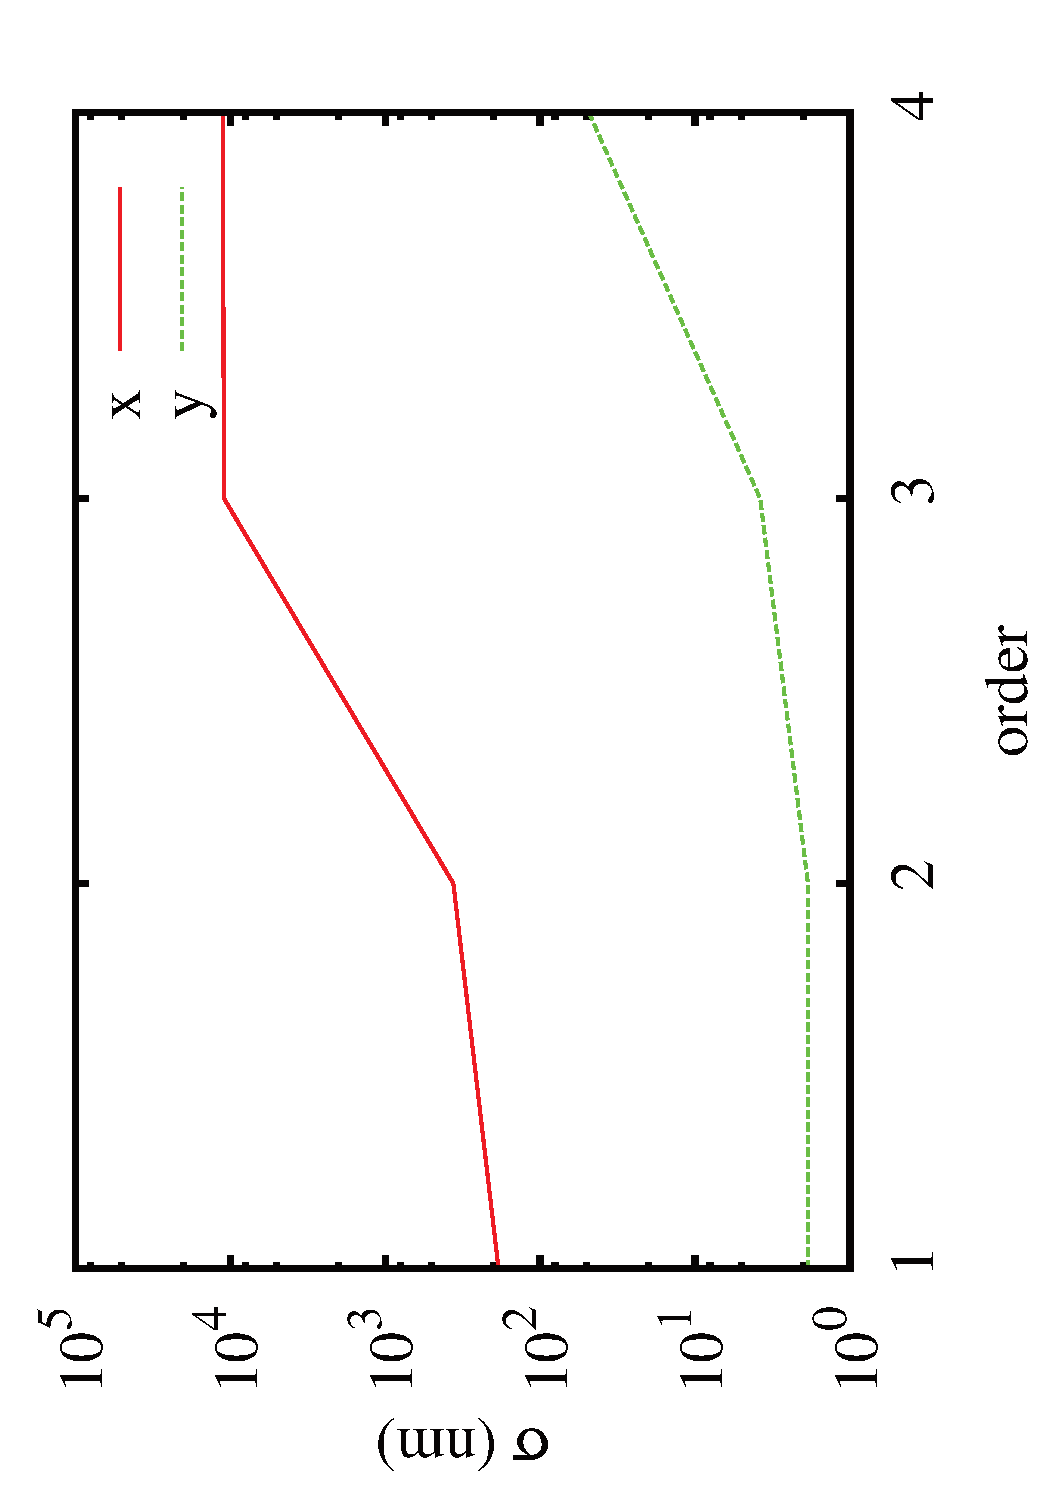
\includegraphics[scale=0.25,angle=-90]{sigmas.pdf}
 \end{textblock}
\vspace*{0.5cm}
The third order terms $U_{1166}$ and $U_{3466}$ increase the beam size due to second order dispersion at the sextupole inside the Final doublet.\par
Second order dispersion needs to be corrected before the FD (not only at the IP) and must remain zero because of the sextupole, or we should tolerate some dispersion in the FD.\par

\vspace*{4cm}
\end{frame}
% \section{Conclusions}
% \begin{frame}{Conclusions}
%  \begin{itemize}
%   \item The distance between the quadrupoles in the FD should be around one and two times the $L^*$.
%   \item Phase advance and beta ratios should be matched with enough precision to allow the geometrical terms cancellation.
%   \item Sextupoles position should be placed to get a phase advance as close to $(2n+1)\pi/2$ as possible.
%   \item A non-interleaved line latice has been created from previous lattice designs and matched to these requirements. As a result, second order components in the vertical beam size were corrected and 25\% horizontal beam size increase was obtained.
%   \item Lattice length reduction, magnets optimization and tunning evaluation is foreseen.
%  \end{itemize}
% \end{frame}
\end{document}